\documentclass{article}
\usepackage{iclr2027_conference,times}

% Optional math commands
\input{math_commands.tex}

\usepackage{hyperref}
\usepackage{url}
\usepackage{booktabs}
\usepackage{multirow}
\usepackage{algorithm}
\usepackage{algpseudocode}
\usepackage{float}
\usepackage{caption}
\usepackage{subcaption}
\usepackage{amsmath}
\usepackage{amssymb}
\usepackage{amsthm}
\usepackage{mathtools}
\usepackage{xcolor}
\usepackage{siunitx}

% Compact float separation (typographic tuning only; no content is affected)
\setlength{\textfloatsep}{10pt plus 2pt minus 2pt}
\setlength{\floatsep}{8pt plus 2pt minus 2pt}
\setlength{\intextsep}{8pt plus 2pt minus 2pt}
\setlength{\abovecaptionskip}{6pt}
\setlength{\belowcaptionskip}{2pt}

% Theorems (using ICLR style)
\newtheorem{theorem}{Theorem}[section]
\newtheorem{lemma}[theorem]{Lemma}
\newtheorem{corollary}[theorem]{Corollary}
\newtheorem{definition}{Definition}[section]
\newtheorem{proposition}[theorem]{Proposition}

\title{A2A-BFT: Byzantine Fault-Tolerant Consensus for Agent-to-Agent Protocols}

\author{
  Anonymous Author \\
  Affiliation \\
  \texttt{anonymous@institution.edu} \\
  \AND
  Co-author \\
  Affiliation \\
  \texttt{coauthor@institution.edu}
}


\begin{document}

\maketitle

\begin{abstract}
Agent-to-Agent (A2A) protocols let autonomous agents collaborate on complex tasks, but reliable consensus in heterogeneous agent networks remains a fundamental challenge once Byzantine failures and soft faults are admitted. We propose \textbf{A2A-BFT}, a Byzantine fault-tolerant consensus extension for A2A protocols: a three-phase semantic consensus protocol (Propose--Validate--Commit) with attack-adaptive decision thresholds and a reputation tracker provably excluded from the vote-counting rule. We prove safety and liveness under $n \geq 3f + s + 1$ ($f$ Byzantine, $s$ soft faults, $s \le f$) and evaluate entirely on real LLM inference: a 7{,}750-task fault sweep with four heterogeneous open-source models ($n{=}250$ per cell) spanning mathematical reasoning, code generation, and knowledge QA. On execution-validated code tasks the protocol \emph{never} commits a wrong answer within the safety boundary ($0.0 \pm 0.0\%$ under every attack), while sub-boundary settings violate safety up to $72.4\%$ on GSM8K and $90.0\%$ on knowledge QA, confirming $3f{+}s{+}1$ as a tight operating condition for $s \le f$; on semantically validated tasks, safety composes with the validation oracle. Under collusion, unvalidated majority-voting and debate baselines commit incorrect answers in $16.7$--$63.4\%$ of tasks \emph{within} the boundary. Ablations identify view change as the core liveness component---removing it collapses decisions from $74.4\%$ to $4.5\%$ under strategic rejection---and dynamic thresholds as the safeguard against attack-induced deadlock. A measured audit shows the released reputation tracker to be decision-neutral but mis-specified as a deterrent: in the four attacked cells, $1{,}186$ of $1{,}305$ aggressive penalties land on honest validators whose vote was objectively correct.
\end{abstract}

\begin{center}
\textbf{Keywords:} Byzantine fault tolerance, agent consensus, large language models, distributed systems, reputation mechanism
\end{center}

\section{Introduction}

Large language models (LLMs) enable autonomous AI agents to perform complex reasoning, code generation, and collaborative problem-solving. The Agent-to-Agent (A2A) protocol, introduced by Google at I/O 2025 and recently donated to the Linux Foundation, provides a standardized framework for inter-agent communication, with over 150 enterprise supporters including Amazon, Anthropic, and Salesforce \citep{a2a_protocol_2025}. Despite these advances, ensuring reliable consensus in multi-agent systems remains an open challenge.

\textbf{Motivating Example:} Consider a collaborative coding task where five agents must agree on a code solution while one agent is compromised (Byzantine fault) or intermittently erroneous (soft fault). Traditional BFT protocols assume deterministic replicas; LLM-based agents introduce stochastic elements that require new consensus mechanisms.

Recent work by ETH Zurich \citep{a2a_sim_2026} found that LLM-based agents reach valid consensus in only 41.6\% of trials \emph{even in benign settings without any Byzantine agents}, with failures dominated by liveness loss rather than value corruption. This gap between theoretical guarantees and practical performance motivates our work: how can a consensus protocol achieve reliability in heterogeneous agent networks whose participants may exhibit Byzantine behaviour, soft faults, or varying capability?

\textbf{Our Approach:} We propose A2A-BFT, a Byzantine fault-tolerant consensus extension with three innovations: (i) a three-phase semantic consensus (Propose-Validate-Commit) tailored to LLM-based reasoning tasks; (ii) attack-adaptive decision thresholds that prevent attack-induced deadlock (Section~\ref{sec:experiments}); and (iii) formal safety and liveness guarantees under partial synchrony with the fault model $n \geq 3f + s + 1$ (with the standing assumption $s \leq f$). We validate the protocol entirely on real four-model LLM deployments (7{,}750-task fault sweep, $n{=}250$ per cell), showing that (a) execution-validated consensus is mechanically safe within the boundary and that safety violations occur only where the theorem says they may ($3f{+}s{+}1$ violated), and (b) on semantically validated tasks, wrong commits under attack are bounded by the validation oracle's error rate---safety composes with the oracle (Corollary~\ref{cor:oracle}). We additionally isolate the reputation tracker---a decision-neutral design component the theorem excludes from every decision---by direct measurement: replaying instrumented vote streams shows it decision-neutral (as the theorem requires) but, as released, directing in the attacked cells $1{,}186$ of $1{,}305$ aggressive penalties at honest validators whose votes were objectively correct.

\section{Related Work}

\textbf{Byzantine fault tolerance in distributed systems.} Classical BFT protocols such as PBFT~\citep{castro1999practical} assume deterministic, faithfully executing replicas with bounded, known-size faults; Byzantine-robust aggregation in distributed learning~\citep{blanchard2017byzantine} tolerates adversarial gradient contributions but targets numeric aggregation. A2A-BFT instead targets \emph{probabilistic} replicas whose correctness depends on sampled LLM outputs, requiring semantic rather than byte-level validation and a unanimity-style agreement probability $p_h^{\,n-1-f-s}$ (Section~\ref{sec:theory}). The $+s$ term is not a re-badged omission count---an omission fault goes silent and is discountable, whereas a soft fault keeps voting and may err stochastically; Section~\ref{sec:theory} prices this with coefficient $1$ on $s$ (versus $3$ on $f$), worst-case abstention in the safety proof, and the standing assumption $s \leq f$ for REJECT-voting soft faults.

\textbf{Multi-agent consensus with LLMs.} Debate- and voting-based aggregation improves answer quality but offers no guarantee against committed wrong answers under Byzantine agents: our experiments show $16.7$--$63.4\%$ wrong-commit rates for such baselines. Self-aggregation frameworks such as A2A-Sim add confidence filtering but no validation stage. Verifier-guided generation and reranking methods likewise use verification to \emph{rank or filter} candidates; A2A-BFT instead uses it to \emph{gate} commitment. To our knowledge, no prior LLM-consensus protocol states a wrong-commit bound in terms of the validation oracle's error rate; A2A-BFT makes that dependence explicit (Corollary~\ref{cor:oracle}) and measures it. Concurrent robust-aggregation designs offer neither property: confidence-probe weighting \citep{zheng2025rethinking} keeps unvalidated weighted aggregation, and self-anchored filter-and-refine consensus \citep{lee2026robust} commits the majority-filtered answer without a validation oracle. The gap is not hypothetical: even an oracle-assisted debate baseline---one that keeps any solution already passing all tests---still commits wrong answers on $46.7$--$56.7\%$ of MBPP tasks under attack (Appendix~\ref{app:attacks}). It is validation \emph{inside} the commit rule, not robustness of the aggregation weights, that binds wrong commits to the oracle's error rate (extended discussion: Appendix~\ref{app:extrelated}).

\section{System Model}

\subsection{Agent Network Model}

We consider a network of $n$ heterogeneous agents $\mathcal{A} = \{A_1, A_2, \ldots, A_n\}$ operating under the A2A protocol framework. Each agent $A_i$ has a unique decentralized identifier (DID) for authentication, a capability score $g_i$ reflecting its domain expertise, a reputation score $r_i \in [0.1, 1.0]$ updated dynamically, and a participation weight $w_i \in [0.1, 2.0]$ used only when the deployment subsamples validators (it does not enter the vote-counting rule; Section~\ref{sec:reputation}).

\subsection{Fault Model}

We extend the classical BFT fault model to account for both Byzantine and soft faults:
\begin{definition}[Fault Model]\label{def:fault}
A system with $n$ agents is characterized by parameters $(n, f, s)$ where:
\begin{itemize}
    \item $f$: maximum number of Byzantine (malicious) agents, which may vote arbitrarily, including equivocation, coordination, or selective rejection.
    \item $s$: maximum number of soft-fault (unreliable) agents, which vote independently with probability $p_s \in [0.5, 0.9]$ of producing ACCEPT on valid proposals, may ABSTAIN or vote REJECT stochastically, and \emph{do not ACCEPT invalid proposals} (Appendix~\ref{app:softfault} quantifies the relaxation).
    \item Safety condition: $n \geq 3f + s + 1$, with $s \leq f$ when soft faults vote REJECT rather than abstaining (Appendix~\ref{app:softfault}).
\end{itemize}
\end{definition}

Soft faults are non-coordinated: soft-fault agents do not communicate with other faulty agents, and their errors are independent. The coefficient 1 on $s$ (vs. 3 on $f$) reflects the reduced threat: soft faults may abstain or err randomly, but they do not actively undermine consensus. This extends the classical $n \geq 3f + 1$ bound, recovering it when $s = 0$.

\subsection{Task Model}\label{sec:task}

We consider a task $T$ drawn from a distribution $\mathcal{D}$ over a task space $\mathcal{T}$, with a verifiable solution space $\mathcal{S}$ and a ground-truth verification function $V: \mathcal{T} \times \mathcal{S} \to \{0, 1\}$. Tasks include mathematical reasoning, code generation, knowledge-based QA, and logic puzzles.

\section{Protocol Design}

A2A-BFT operates in rounds, each consisting of three phases as illustrated in Figure \ref{fig:consensus_flow}: \textbf{Phase 1: Propose} (the designated primary generates a task solution), \textbf{Phase 2: Validate} (other agents independently verify the proposal), and \textbf{Phase 3: Commit} (agents vote on the verification result; the count score $\phi$ is compared against attack-adaptive thresholds).

\begin{figure}[htbp]
\centering
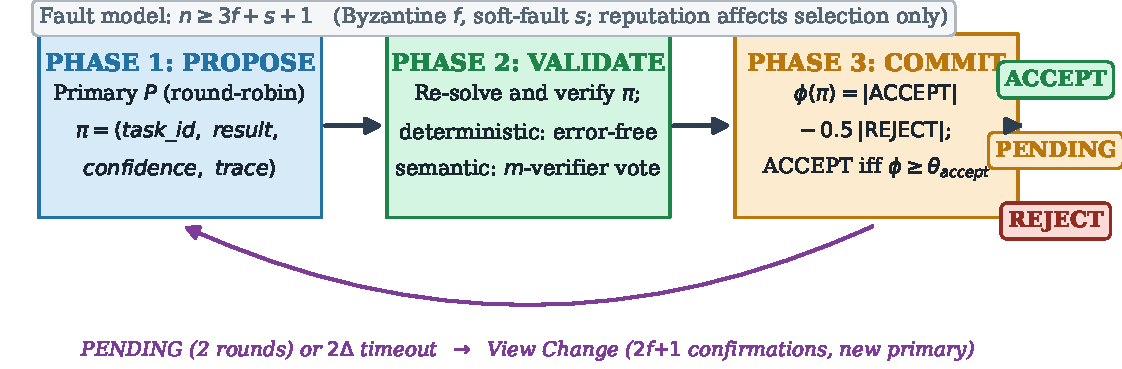
\includegraphics[width=0.78\linewidth]{figures/consensus_flow.pdf}
\caption{A2A-BFT three-phase consensus protocol. The round-robin primary broadcasts a proposal $\pi$ (Phase~1); validators re-solve and verify it---error-free checks for deterministic tasks and $m$-verifier semantic checks otherwise (Phase~2); votes are aggregated by the count score $\phi(\pi)$ under attack-adaptive thresholds (Phase~3). Rejections trigger view change immediately, and PENDING outcomes after two consecutive rounds or a $2\Delta$ timeout.}
\label{fig:consensus_flow}
\end{figure}

\subsection{Phase 1: Propose}

The primary agent $P$ receives task $T$ and produces proposal $\pi = (task\_id, result, confidence, trace)$, where $task\_id$ uniquely identifies the task, $result$ is the proposed solution, $confidence \in [0,1]$ is a self-assessed confidence, and $trace$ is the execution trace for auditability. The proposal is broadcast to all validators with timestamp $\tau$; the primary is selected via round-robin rotation to ensure fairness.

\subsection{Phase 2: Validate}

Each validator $V_i$ independently verifies proposal $\pi$:
\begin{equation}
    \hat{V}_i(\pi) = \begin{cases}
        \text{ACCEPT} & \text{if verification succeeds} \\
        \text{REJECT} & \text{if verification fails} \\
        \text{ABSTAIN} & \text{if verification inconclusive}
    \end{cases}
\end{equation}

Verification re-computes the solution and compares results. Formally, writing $\hat{V}_i$ for validator $i$'s verdict on a proposal (the ground-truth oracle $V$ is defined in Section~\ref{sec:task}), let $\mathrm{ver}(T, s) \in \{0,1\}$ denote whether verification of solution $s$ for task $T$ succeeds: $\mathrm{ver}(T, s) = 1$ iff $s$ matches the ground truth (or an equivalent formulation) in the \emph{execution-validated} domain, where the check is error-free; in the \emph{semantically validated} domain (free-form reasoning and multiple-choice QA), $\mathrm{ver}(T, s) = 1$ iff at least $k$ of $m$ verifiers agree \citep{zheng2023llm}, with $k = \lceil 2m/3 \rceil$; the verifier error then falls to the binomial tail $\sum_{j=0}^{k-1}\binom{m}{j}p_h^{\,j}(1-p_h)^{m-j}$ rather than $(1-p_h)^m$, where $p_h$ is the probability that an honest validator correctly accepts a valid proposal. In our experiments code generation (MBPP) is execution-validated while mathematics (GSM8K) and knowledge QA (MMLU) are semantically validated, each validator using a \emph{single} self-model judge ($m{=}1$), so redundancy comes \emph{across} validators via Phase~3; a mild self-preference bias is possible when a validator shares the primary's model \citep{zheng2023llm}, though one-model-per-replica makes this rare. The released judge emits a discrete verdict, ABSTAIN marking an explicit UNCERTAIN outcome (the band $[0.4, 0.6]$ on a calibrated probability); an ABSTAIN contributes 0 to $\phi(\pi)$.

This tail decays exponentially only once $k/m$ is held fixed: the ceiling in $k = \lceil 2m/3\rceil$ makes small-$m$ choices non-monotone ($0.028$ at $m{=}3$ but $0.0815$ at $m{=}5$ for $p_h = 0.9$), so deployments should pick $m$ as a multiple of three. In general, $m > 1$ trades additional inference cost for lower verification error.

\subsection{Phase 3: Commit}

Validators broadcast votes $vote_i = (\hat{V}_i(\pi), signature_i)$ to all agents, with $v_i \in \{-1, 0, 1\}$ encoding REJECT=$-1$, ABSTAIN=$0$, ACCEPT=$+1$ over the validator set $\mathcal{V}$ (excluding the primary). The consensus aggregator computes vote count score:

\begin{equation}
    \phi(\pi) = |\{i : v_i = \text{ACCEPT}\}| - 0.5 \cdot |\{i : v_i = \text{REJECT}\}|
\label{eq:commit}
\end{equation}

\textbf{Consensus Decision:}
\begin{equation}
    Decision(\pi) = \begin{cases}
        \text{ACCEPT} & \text{if } \phi(\pi) \geq \theta_{accept} \\
        \text{REJECT} & \text{if } \phi(\pi) \leq \theta_{reject} \\
        \text{PENDING} & \text{otherwise}
    \end{cases}
\end{equation}

with dynamic thresholds:
\begin{align}
    \theta_{accept} &= n - 1 - 2f - s \\
    \theta_{reject} &= -(n - 1 - f) \cdot 0.5
\end{align}

where the threshold is derived from the safety condition $n \geq 3f + s + 1$. This ensures that if all honest validators accept, the proposal passes even with $f$ Byzantine validators rejecting (and, when soft faults also reject, provided $s \leq f$; Appendix~\ref{app:softfault}).

\subsection{Reputation Mechanism}
\label{sec:reputation}

A2A-BFT maintains per-agent reputation scores $r_i \in [0.1, 1.0]$ updated each round. Algorithm~\ref{alg:reputation} tiers penalties by the historical rejection ratio $\rho_i$ over a 10-round window; vote correctness is judged against \emph{proposal quality} ($c$), not the committee's final decision, so a validator that correctly rejects a wrong proposal is \emph{specified} to be rewarded even if the majority accepts it. Section~\ref{sec:rep_ablation} measures whether the released implementation actually delivers this (it does not) while leaving every commit decision untouched.

\begin{algorithm}[t]
\caption{Reputation Update with Tiered Penalties}
\label{alg:reputation}
\begin{algorithmic}[1]
\Require Reputation $r_i$; vote $v_i$; proposal correct? $c$; reject ratio $\rho_i$ (10-round window)
\Ensure Updated reputation $\hat{r}_i$
\State $\text{ok} \gets (v_i = \textsc{Accept} \wedge c) \vee (v_i = \textsc{Reject} \wedge \neg c)$ \Comment{ABSTAIN is never ``correct''}
\If{$\rho_i \geq 0.7$} \Comment{persistent rejecter}
    \State $\hat{r}_i \gets \max(0.1,\, r_i - 0.25)$
\ElsIf{$\text{ok} \wedge \rho_i < 0.5$} \Comment{correct vote}
    \State $\hat{r}_i \gets \min(1.0,\, r_i + 0.1)$
\ElsIf{$\neg \text{ok}$} \Comment{honest mistake}
    \State $\hat{r}_i \gets \max(0.5,\, r_i - 0.05)$
\Else \Comment{neutral drift}
    \State $\hat{r}_i \gets \max(0.5,\, r_i - 0.02)$
\EndIf
\State \textbf{return} $\hat{r}_i$
\end{algorithmic}
\end{algorithm}

The reputation score is an incentive and accountability signal, not an input to the vote-counting rule: Equation~\ref{eq:commit} aggregates raw vote \emph{counts}, so reputation cannot alter a commit decision---the sweep runs with uniform weights ($w_i{=}1$) and contains no reputation logic in its consensus path (Section~\ref{sec:experiments}), so no reported decision depends on this component. The reference implementation maintains per-agent scores, a 10-round voting history, and suspect counters, and escalates penalties for persistent misbehaviour (Algorithm~\ref{alg:reputation}); weighting validator selection and excluding persistent offenders are specified extensions the released code does \emph{not} realise, and no deployment here subsamples validators. The tiered structure (aggressive $-0.25$ for persistent rejecters, reward $+0.1$ for correct votes, mild $-0.05$ for honest mistakes, neutral drift $-0.02$) is \emph{intended} to provide graduated deterrence against strategic rejection; Section~\ref{sec:rep_ablation} measures how far the released trigger falls short of that intent. ABSTAIN is never ``correct'': the predicate of Algorithm~\ref{alg:reputation} is a disjunction, since the form $(v_i = \textsc{Accept}) = c$ would score abstention on an \emph{incorrect} proposal as correct and could pay the reward for it (Section~\ref{sec:rep_ablation}).

\subsection{View Change Protocol}

When the primary fails, when a proposal is rejected, after two consecutive PENDING rounds, or on a $2\Delta$ timeout, a view change is triggered:
\begin{enumerate}
    \item Any honest agent may initiate view change after $2\Delta$ timeout.
    \item Propose VIEW-CHANGE message with new view number.
    \item Collect $2f+1$ confirmations to establish new primary.
    \item Switch to new primary and resume consensus.
\end{enumerate}
Safety across views holds because the primary of each view number is fixed by deterministic round-robin order, any $2f{+}1$ confirmation quorum contains at least $f{+}1$ non-Byzantine agents---hence at least $f{+}1{-}s \geq 1$ strictly honest ones (non-Byzantine is weaker than honest when soft faults exist)---and the at most $f$ Byzantine agents cannot establish a view; a committed task terminates its instance. Cross-view state transfer and the assumptions it rests on are detailed in Appendix~\ref{app:viewchange}.

\subsection{Alternative Proposal Handling}\label{sec:altprop}

When a proposal is rejected or times out, secondary validators may submit competing proposals, which enter the PENDING state for consideration in the next round, with priority given to higher-confidence submissions.

\section{Theoretical Analysis}
\label{sec:theory}

\subsection{Safety Theorem}

\begin{theorem}[Safety]
\label{thm:safety}
Under $n \geq 3f + s + 1$, DID-authenticated channels, single-proposal broadcast with consistent dissemination of honest votes, and worst-case soft-fault abstention, A2A-BFT satisfies: (i) \emph{decision consistency}: no two honest validators reach \emph{opposite} terminal decisions on the same proposal, and honest replicas may differ only between ACCEPT and PENDING, which the commit broadcast or view change resolves; and (ii) \emph{commit validity}: within the boundary a wrong commit requires an honest validation error (or a wrong honest-primary proposal), whereas below the boundary Byzantine validators alone can commit a tampered proposal.
\end{theorem}

\begin{proof}[Proof sketch]
(i) Honest replicas share the same honest votes, so scores differ only through Byzantine vote equivocation, which the threshold gap provably absorbs ($\theta_{accept}-\theta_{reject} \geq 2f+0.5s > 1.5f$; Appendix~\ref{app:proofs}); opposite terminal decisions are therefore impossible, and ACCEPT-vs-PENDING divergence resolves through the commit broadcast or view change. Proposals carry the primary's DID signature, and conflicting signed proposals from one primary trigger a view change that voids the round, so equivocation cannot yield two concurrent acceptances. (ii) Byzantine validators number at most $f-1$ when the primary is Byzantine ($f$ otherwise) and contribute $+1$ each, so commitment requires at least $\theta_{accept}-(f{-}1) = n{-}3f{-}s \geq 1$ honest ACCEPT votes when the primary is Byzantine, and $\theta_{accept}-f = n{-}1{-}3f{-}s \geq 0$ otherwise. Within the boundary, then, a wrong proposal cannot be committed through Byzantine votes alone---it needs an honest validation error or a wrong honest-primary proposal, both bounded by oracle reliability $p_h$ (Section~6). Below the boundary the implication fails instead through the honest validators' own REJECTs: a non-tampering primary's wrong proposal, rejected by $n{-}1{-}f{-}s$ honest validators (soft faults abstaining, the worst case) against $f$ Byzantine ACCEPTs, clears $\theta_{accept}$ exactly when $7f + 3s + 3 \geq 3n$, matching Table~\ref{tab:bft}. Full proof in Appendix~\ref{app:proofs}. \qed
\end{proof}

\begin{corollary}[Oracle composition]
\label{cor:oracle}
Within the boundary, every committed wrong answer implies a validation-oracle error (claim~(ii) of Theorem~\ref{thm:safety}), so the wrong-commit rate is bounded by the oracle's error probability---zero under a perfect oracle.
\end{corollary}

\subsection{Liveness Theorem}

\begin{theorem}[Liveness]
\label{thm:liveness}
Under partial synchrony, $n \geq 3f + s + 1$, and the standing assumption $f \geq s$, A2A-BFT reaches a decision (ACCEPT or REJECT) for any valid task proposal with probability $1$---\emph{including} under sustained coordinated rejection of every honest proposal by the Byzantine validators. Coordinated rejection blocks termination only if soft faults vote REJECT (rather than abstain) and $f < s$.
\end{theorem}

\begin{proof}[Proof sketch]
The primary rotates round-robin, so an honest agent becomes primary within every $f+1$ rounds. With an honest primary, a sufficient event for acceptance is that all $(n-1-f-s)$ honest validators accept; Lemma~\ref{lem:acceptance} lower-bounds the single-round acceptance probability by $p_h^{(n-1-f-s)} = 0.81$ for $n{=}5, f{=}1, s{=}1$ ($p_h = 0.9$). Crucially, this event survives coordinated rejection: all-honest-accept with soft faults abstaining (the worst-case convention of Theorem~\ref{thm:safety}) gives $\phi - \theta_{accept} = 0.5f \geq 0$ \emph{regardless of the Byzantine votes}. If the decision is PENDING, view change (requiring $2f+1$ confirmations, more than the $f$ Byzantine agents) rotates the primary within $f+1$ further rounds. After GST, the probability of no acceptance within $k$ honest-primary rounds is bounded by $(1 - p_h^{(n-1-f-s)})^k$, so termination occurs with probability $1$; the same bound justifies the round-bounded decision rates of Section~\ref{sec:experiments}. The assumption $f \geq s$ enters only when soft faults vote REJECT; if additionally $f < s$, sustained coordinated rejection can block acceptance---the sole case outside the guarantee. Full proof in Appendix~\ref{app:proofs}. \qed
\end{proof}

\begin{lemma}[Acceptance Probability Bound]
\label{lem:acceptance}
For $n \geq 3f + s + 1$ and honest primary, the probability of acceptance in a single round is at least $p_h^{(n-1-f-s)}$.
\end{lemma}

\begin{proof}
When the primary is honest, it generates a valid proposal. Each honest validator independently accepts with probability $p_h$. Since there are $(n-1-f-s)$ honest validators, the probability that all accept is $p_h^{(n-1-f-s)}$. All-accept ensures $\phi \geq \theta_{accept}$ under the stated abstention behaviour of soft faults; if the $f$ Byzantine \emph{and} $s$ soft-fault validators all vote REJECT the implication requires $f \geq s$, as assumed throughout (Appendix~\ref{app:softfault}). \qed
\end{proof}

\subsection{Complexity Analysis}
Table \ref{tab:complexity} (Appendix~\ref{app:implementation}) compares message complexity with representative BFT protocols. A2A-BFT keeps $O(n^2)$ messages per round, like PBFT, and bounds expected rounds in practice ($2.6$--$4.5$ measured, Table~\ref{tab:performance}) via attack-adaptive thresholds and view-change rotation.

\section{Experimental Evaluation}
\label{sec:experiments}

\subsection{Experimental Setup}\label{sec:setup}

\textbf{Reproducibility:} All protocol-level fault-tolerance experiments share one heterogeneous four-model deployment with 5 seeds and 50 tasks per (configuration, seed, dataset), i.e., $n{=}250$ per cell (7{,}750 tasks over 31 cells); task sets are drawn per seed by a seeded shuffle over GSM8K \citep{gsm8k}, MBPP \citep{mbpp}, and MMLU \citep{mmlu} and reused across configurations for paired comparison. \textbf{No simulation:} every reported number comes from real LLM inference ($7{,}750$ fault sweep + $4{,}320$ ablation/baseline + $770$ API tasks); seeds, models, hardware, injection, and the reputation measurement are specified in the Reproducibility Statement and Appendix~\ref{app:attacks}.

\textbf{Statistical Methodology:} results are reported as mean $\pm$ standard deviation over seeds with 95\% Wilson score intervals on pooled task counts; rounds are compared by two-sided Welch $t$-tests and decision rates by the exact McNemar test, both over identical per-task sampling.

\subsection{Baseline Results}

Table \ref{tab:baseline} (Appendix~\ref{app:additional}) shows baseline performance without Byzantine faults.

\textbf{Note on decision semantics:} a task is \emph{decided} when a proposal is committed within the 6-round bound (rejections and PENDING rounds trigger view change and retry); \emph{wrong-commit} counts tasks committed with an incorrect answer. Under semantic validation the single-round acceptance bound $p_h^{\,n-1-f-s}$ keeps the fault-free decision rate at $55$--$59\%$ on GSM8K---heterogeneous replicas disagree often, and the protocol refuses to commit when validation is inconclusive; on MBPP, where validation executes all test assertions, it is $70$--$74\%$ with \emph{zero} wrong commits.

\subsection{Byzantine Fault Tolerance}
Table \ref{tab:bft} reports consensus performance under the three Byzantine attack types across fault configurations.

\begin{table}[htbp]
\centering\small
\caption{BFT Performance Under Attack (real heterogeneous 4-model deployment; cells: decision\% / wrong-commit\%, mean$\pm$std over sampling seeds; $n{=}250$ per cell except the $n{=}5, f{=}1, s{=}1$ strategic-reject row, $n{=}90$, from Table~\ref{tab:ablation}, Appendix~\ref{app:additional}). Bold marks the \emph{best} (lowest) wrong-commit rate per column. $^\dag$: configuration below the safety boundary $3f{+}s{+}1$ ($n \geq 7$ required for $f{=}2$). MMLU results in Table~\ref{tab:mmlu_sweep}.}
\label{tab:bft}
\begin{tabular}{ccclcccc}
\toprule
\textbf{n} & \textbf{f} & \textbf{s} & \textbf{Attack} & \multicolumn{2}{c}{\textbf{GSM8K (semantic)}} & \multicolumn{2}{c}{\textbf{MBPP (execution)}} \\
\cmidrule(lr){5-6} \cmidrule(lr){7-8}
 & & & & decision & wrong & decision & wrong \\
\midrule
4 & 1 & 0 & Random & $90.8 \pm 3.0$ & $14.0 \pm 4.0$ & $73.6 \pm 6.5$ & $\mathbf{0.0 \pm 0.0}$ \\
4 & 1 & 0 & Strat.\ Reject & $80.8 \pm 3.6$ & $23.2 \pm 7.0$ & $71.2 \pm 6.4$ & $\mathbf{0.0 \pm 0.0}$ \\
4 & 1 & 0 & Sybil & $90.4 \pm 3.3$ & $12.8 \pm 4.4$ & $73.6 \pm 6.5$ & $\mathbf{0.0 \pm 0.0}$ \\
5 & 1 & 1 & Random & $89.2 \pm 3.0$ & $11.6 \pm 3.8$ & $73.2 \pm 7.2$ & $\mathbf{0.0 \pm 0.0}$ \\
\textbf{5} & \textbf{1} & \textbf{1} & \textbf{Strat.\ Reject} & $\mathbf{74.4 \pm 8.4}$ & $\mathbf{4.5 \pm 3.9}$ & $70.0 \pm 11.5$ & $\mathbf{0.0 \pm 0.0}$ \\
5 & 2 & 0 & Random$^\dag$ & $96.8 \pm 3.6$ & $22.0 \pm 5.5$ & $78.8 \pm 6.1$ & $5.6 \pm 1.7$ \\
5 & 2 & 0 & Strat.\ Reject$^\dag$ & $95.2 \pm 2.3$ & $67.6 \pm 7.4$ & $74.4 \pm 6.2$ & $9.6 \pm 1.7$ \\
5 & 2 & 0 & Collusion$^\dag$ & $98.4 \pm 1.7$ & $72.4 \pm 5.0$ & $75.6 \pm 4.8$ & $9.2 \pm 5.0$ \\
6 & 2 & 0 & Collusion$^\dag$ & $82.4 \pm 3.3$ & $25.2 \pm 1.8$ & $66.4 \pm 4.8$ & $\mathbf{0.0 \pm 0.0}$ \\
\bottomrule
\end{tabular}
\end{table}

Three findings emerge. \textbf{(i) Safety is exactly as strong as the validation oracle, and the boundary is tight.} On MBPP, every configuration within the safety boundary commits a wrong answer in $\mathbf{0.0 \pm 0.0\%}$ of tasks ($n{=}250$/cell; zero events, corresponding to a pooled $95\%$ Wilson upper bound of $1.5\%$ per cell) regardless of attack, whereas all $n{=}5, f{=}2$ configurations below the boundary violate safety ($5.6$--$9.6\%$), where $\theta_{accept} = 0$ lets two Byzantine ACCEPTs offset the honest REJECTs of a non-tampering primary's wrong proposal. \textbf{(ii) On semantic domains, eventual acceptance trades safety for liveness under sustained attack.} GSM8K wrong commits rise to $11.6$--$23.2\%$ within the boundary: a Byzantine primary submits a plausible-but-wrong answer, weak 8B judges accept it with non-negligible probability, and retry semantics keep sampling until one passes validation---the system \emph{does} decide ($74$--$91\%$) but inherits the judge's error rate. \textbf{(iii) Decision rates rise under attack} (up to $98\%$ vs.\ $59.2\%$ fault-free): Byzantine primaries inject extra proposals that eventually clear validation, so we report wrong commits as the primary safety metric.

\subsection{Real LLM Validation (Homogeneous Upper Bound)}

As a complementary check we validated the protocol with real DeepSeek-V2-Lite outputs over 320 tasks spanning GSM8K, MMLU, and MBPP. These runs use a \emph{homogeneous} single-model deployment, so honest validators agree far more often than in the heterogeneous sweep; the resulting $100\%$ acceptance across all eight configurations, under strategic rejection and collusion alike, is therefore an \emph{upper bound} on decision rates rather than a contradiction of the $55$--$74\%$ heterogeneous results. At the boundary configuration $n{=}8, f{=}2, s{=}1$ (150 GSM8K tasks per configuration, real DeepSeek API), the protocol maintains $98$--$100\%$ consensus under both attacks across two independent runs, with answer correctness within $2$ points of the fault-free baseline ($92.0$--$92.7\%$ vs.\ $94.0\%$), and the round-count gap versus fault-free ($1.03$ vs.\ $2.89$--$2.92$) confirms genuine attack resistance (Welch $t = -13.1$ and $-13.9$, $p < 10^{-26}$; reproduced at $1.04$ vs.\ $2.38$--$2.43$, McNemar exact $p = 0.25$). Details: Appendix~\ref{app:realllm}; scaling and MMLU sweeps: Appendix~\ref{app:additional}.

\subsection{Ablation Study}

To isolate each protocol component we ablate in the \emph{heterogeneous four-model} setting (Section~\ref{sec:setup} models, one per replica, vLLM on two A800 GPUs) on two domains with different validation semantics: \emph{GSM8K}, where Validate uses an independent LLM judge, and \emph{MBPP}, where Validate executes the submitted code against test assertions---in verifiable domains a wrong commit is mechanically impossible for the full protocol. Each scenario uses 30 tasks per seed over three seeds ($42/43/44$; $90$ per scenario); Byzantine validators employ strategic rejection ($n{=}5, f{=}1, s{=}1$) or collusion ($n{=}8, f{=}2, s{=}1$). Soft faults exercise the abstention arm (ABSTAIN w.p.\ $0.3$; Appendix~\ref{app:softfault})---the stochastic-REJECT arm of Definition~\ref{def:fault} is analysed, not injected. Table~\ref{tab:ablation} (Appendix~\ref{app:additional}) reports decision rates and wrong-commit rates.


The ablation yields four consistent findings. \textbf{(i) View change is the core liveness component:} removing it collapses decisions from $74.4 \pm 8.4\%$ to $4.5 \pm 3.9\%$ (GSM8K, strategic rejection) and to $0\%$ (MBPP, both attacks)---blocked rounds never rotate the primary, confirming Theorem~\ref{thm:liveness}. \textbf{(ii) Semantic validation is the prerequisite for heterogeneous consensus:} under naive exact-match comparison, heterogeneous replicas almost never agree byte-for-byte, so valid proposals are rejected indefinitely and the code domain deadlocks ($0$--$1.1\%$ decisions)---Validate must be semantic, not syntactic. On GSM8K, dropping semantic validation \emph{lowers} wrong commits ($2.2 \pm 1.9\%$ vs.\ the full protocol's $4.5 \pm 3.9\%$; conditional on deciding, $4.0\%$ vs.\ $6.0\%$)---as Corollary~\ref{cor:oracle} predicts: the exact-match oracle rarely commits and so rarely errs, while the LLM-judge oracle commits more often ($54.4\% \to 74.4\%$) and inherits the judge's error rate in exchange; both rates remain bounded by their respective oracle errors. \textbf{(iii) Dynamic thresholds prevent attack-induced deadlock:} a fixed majority threshold drives every strategic-rejection round on GSM8K into the pending region ($0.0 \pm 0.0\%$, all seeds), whereas attack-adaptive thresholds restore $74.4 \pm 8.4\%$. \textbf{(iv) Safety is preserved:} at most $10.0 \pm 3.3\%$ wrong commits on GSM8K and \emph{never} on MBPP (pooled $95\%$ Wilson interval $[0.0, 4.1]\%$ at $n{=}90$)---on execution-validated domains every committed solution passes all test assertions by construction.

\textbf{Comparison with baselines under Byzantine attacks.} Table~\ref{tab:hetero_compare} (Appendix~\ref{app:additional}) evaluates the full protocol against four baseline aggregation strategies in the same heterogeneous environment (operational definitions in Appendix~\ref{app:attacks}).


Three observations follow. \textbf{First, high decision rates are not safety.} All voting- and debate-based baselines decide on every task, yet under collusion commit incorrect answers in $16.7$--$63.4\%$: unvalidated majority voting converts Byzantine injections and honest errors into committed consensus, whereas the full protocol forgoes such decisions ($60$--$74\%$ decision rates under attack). \textbf{Second, unverified debate amplifies attacks:} LLM-Debate \citep{du2024improving} is the least safe on code ($63.4 \pm 5.8\%$ wrong commits under collusion), because debate without a verification oracle lets Byzantine agents drag honest replicas toward corrupted solutions. \textbf{Third, the correct-when-decided gap matters:} conditioned on committing, A2A-BFT reaches $83$--$100\%$ answer correctness across all eight attacked scenarios versus $37$--$89\%$ for the baselines; against A2A-Sim, our GSM8K wrong-commit rates are within noise (descriptive only at three seeds), but A2A-Sim decides fewer tasks ($62.2\%$ vs.\ $74.4\%$) and collapses on code ($34.4$--$35.5\%$ against our $0.0{\pm}0.0$).

\textbf{Note on evaluation budget.} Baselines commit in a single round while A2A-BFT may retry for up to six view-change-driven rounds; under the same budget, the oracle-assisted debate baseline still commits wrong answers on $46.7$--$56.7\%$ of MBPP tasks, so the safety gap is not a pure budget effect (Appendix~\ref{app:attacks}).

\subsection{Reputation Tracker: Measured Behaviour}\label{sec:rep_ablation}

The tracker does not enter the vote-counting rule (Equation~\ref{eq:commit}), so it cannot change a commit decision---a consequence of Theorem~\ref{thm:safety}, not a finding. We instead measure \emph{what the tracker reports}: we logged every validation vote from the four-model deployment (120 runs, 457 scored proposal rounds, 2{,}461 validation events) and replayed them offline through Algorithm~\ref{alg:reputation} under four settings ($c$ from ground truth or the released heuristic; reputation persisting or reset per task; Appendix~\ref{app:rep_details}). Decision-neutrality is \emph{checked} rather than assumed: recomputing $\phi$ from the raw votes reproduces all $457$ recorded rounds; replaying the vote-and-threshold state machine reproduces all $120$ decisions with primary rotation; injecting reputation weights shifts $\phi$ in up to $421$ rounds and flips up to $5$ decisions, so the check can fail (Appendix~\ref{app:rep_details}).

The measured behaviour is negative. \textbf{(i) The aggressive tier fires on honest, correct votes:} across the four attacked cells, $1{,}186$ of $1{,}305$ aggressive penalties ($\rho_i \geq 0.7$) landed on an honest validator whose vote was \emph{objectively correct}---the behaviour Section~\ref{sec:reputation} specifies should be rewarded---and \emph{all 20 tasks} in each attacked cell produced at least one mis-penalty. \textbf{(ii) As a Byzantine detector the tier fails:} precision $0.232$/$0.195$ (recall $1.000$) under strategic rejection but precision \emph{and} recall $0.000$ under collusion: a colluder rejects only in the commit round and never reaches $\rho = 0.7$, whereas honest validators rejecting those same primaries' wrong proposals do. \textbf{(iii) The score ordering inverts:} honest validators finish \emph{below} Byzantine ones in both collusion cells ($0.337$ vs.\ $0.427$ on GSM8K; $0.300$ vs.\ $0.412$ on MBPP), and resetting reputation per task does not repair this ($0.391$ vs.\ $0.761$)---structural, not a cold-start artefact. \textbf{(iv) The released $c$ carries negative information:} \texttt{\_estimate\_correctness} is a per-domain constant (always \texttt{False} on GSM8K, \texttt{True} on MBPP) agreeing with ground truth on $46.2\%$ of rounds---worse than the trivial always-\texttt{False} predictor ($74.6\%$)---so the promised reward for correct rejection never occurs.

This failure mode is known to the trust literature \citep{josang2002beta,josang2007survey,kamvar2003eigentrust}; what we add is its scale in a real LLM consensus deployment and evidence that it is structural. Because no reported safety or liveness \emph{number} depends on the tracker, the quantitative results stand, but the deterrent listed in Appendix~\ref{app:attack_resistance} should be read as specified rather than realised. A repaired trigger needs a correctness oracle for \emph{proposal} quality and a key not tied to the validator's own rejection ratio (Appendix~\ref{app:rep_details}); the released vote streams and replay make any such repair measurable the same way.



\textbf{Limitations.} A2A-BFT assumes DID-authenticated channels (Ed25519), and consensus quality depends on LLM capability: the fault-free decision rates ($55$--$59\%$ GSM8K, $11$--$15\%$ MMLU; Table~\ref{tab:mmlu_sweep}) imply weaker validation reliability on semantic domains, which the lower-bound form of Lemma~\ref{lem:acceptance} accommodates. The implementation scales to $n \leq 10$; ablation cells ($n{=}90$) limit power for fine-grained comparisons though the reported contrasts far exceed sampling noise; the tracker is decision-neutral but mis-specified (Section~\ref{sec:rep_ablation}; single sampling seed, 20 tasks per cell); the MMLU collapse reflects model capability, not the protocol. Privacy: Appendix~\ref{sec:discussion}.

\section{Conclusion}

We presented A2A-BFT, a Byzantine fault-tolerant consensus protocol for Agent-to-Agent collaboration with provable safety and liveness under $n \geq 3f + s + 1$ ($s \leq f$). A fully real-LLM evaluation (7{,}750-task four-model fault sweep, $n{=}250$/cell, plus ablation and baseline studies) shows liveness under every evaluated attack and safety that binds where the theory predicts: zero wrong commits on execution-validated tasks within the boundary, violations below it, and oracle-bounded wrong commits on semantic tasks. Implications, privacy, and related work: Appendix~\ref{sec:discussion}.

\subsection*{AI Use Statement}
In this work, we used generative AI tools for code development and documentation writing. We have reviewed all AI-assisted work and take responsibility for the final content of this work, including all text, claims, and artifacts.

\subsection*{Reproducibility Statement}
All source code, experimental data, and model configurations are available at \url{https://github.com/anonymous/a2a-bft} (anonymized for review). Section~\ref{sec:setup} summarises the setup; in full, all protocol-level fault-tolerance runs use the same heterogeneous four-model deployment with 5 seeds ($\{42, 43, 44, 45, 46\}$) and 50 tasks per (configuration, seed, dataset) ($n{=}250$ per cell; 7{,}750 tasks over 31 cells), with task sets drawn per seed by a seeded shuffle over GSM8K, MBPP, and MMLU and reused across configurations for paired comparison, while ablation and baseline comparisons use 3 seeds ($\{42, 43, 44\}$) with $n{=}90$ per cell. The four models (Llama-3.1-8B, DeepSeek-V2-Lite, InternLM3-8B, Qwen2.5-7B; Instruct/Chat variants) are served by vLLM \citep{vllm} $0.11$ (temperature $0$, max\_tokens $512$) on two NVIDIA A800-SXM4-80GB GPUs (CUDA 12.8, PyTorch 2.8.0). No simulated workers are used anywhere: every reported number comes from real LLM inference---7{,}750-task fault sweep; $4{,}320$ ablation/baseline tasks ($48$ cells $\times$ $90$); and $770$ API tasks ($320$ multi-domain validation, Table~\ref{tab:real_llm}, and $450$ adversarial-boundary scaling, Table~\ref{tab:n8_scaling}). Of the $48$ ablation/baseline cells, $36$ are tabulated (Tables~\ref{tab:ablation} and~\ref{tab:hetero_compare}); the remaining $12$ are fault-free baseline-condition pairings retained in the released aggregates. The reputation-tracker measurement of Section~\ref{sec:rep_ablation} additionally releases the fully instrumented vote streams (\texttt{reputation\_vote\_stream.json}) for 120 consensus tasks ($6$ cells $\times$ $20$), the two-phase measurement-and-replay script, the decision-neutrality audit (which recomputes the tally from raw votes, reproduces the recorded decisions, and mutation-tests its own resolution), and the fidelity audit against the released penalty code, so that every reported tracker quantity can be recomputed offline without any LLM calls; those quantities are event counts, reported without a variance.

\bibliography{references}
\bibliographystyle{iclr2027_conference}

\appendix
\section{Appendix}

\subsection{Proof Details}

Additional proof details and extended theorems are provided in this appendix.

\subsubsection{Reputation Weights and Safety}

The Safety Theorem (Theorem~\ref{thm:safety}) is stated for the unweighted vote count $\phi(\pi)$, and this is the rule the reference implementation uses: reputation scores $r_i$ never enter Equation~\ref{eq:commit}. Reputation affects only (i) the score update and penalty schedule of Algorithm~\ref{alg:reputation} and (ii) the suspect counters used for anomaly detection (Section~4.4); it does not appear in Equation~\ref{eq:commit}. Selection weights $w_i = w^{\text{base}}_i \cdot \max(r_i, 0.3) \in [0.1, 2.0]$ and exclusion of persistent offenders are specified for deployments that subsample validators; \emph{the released implementation contains neither, and no experiment in this paper subsamples validators}. Since the consensus decision aggregates raw vote counts, the proof of Theorem~\ref{thm:safety} applies unchanged. We deliberately do not analyze a weighted-vote variant here: weighting votes by $w_i$ would couple the threshold analysis to reputation dynamics and require re-deriving $\theta_{accept}$; we leave that variant, which trades a stronger incentive channel for a more complex safety argument, as future work.

\subsubsection{Soft Fault Adversarial Behavior}\label{app:softfault}

Theorem~\ref{thm:safety} assumes soft-fault agents abstain in the worst case (Definition~\ref{def:fault} additionally excludes false-positive ACCEPT votes on invalid proposals, which the analysis below relaxes). If soft-fault agents vote adversarially (REJECT on valid proposals), the minimum vote count becomes:
\begin{equation}
    \phi_{min}^{\text{adversarial}} = (n - 1 - f - s) - 0.5f - 0.5s = n - 1 - 1.5f - 1.5s
\end{equation}
Substituting $n = 3f + s + 1$:
\begin{equation}
    \phi_{min}^{\text{adversarial}} = 1.5f - 0.5s
\end{equation}
For $s = 0$, this equals $1.5f > f = \theta_{accept}$. For $s > 0$, the bound weakens but $\phi_{min}^{\text{adversarial}} = 1.5f - 0.5s \geq f = \theta_{accept}$ whenever $s \leq f$, with strict inequality for $s < f$. Thus, the safety condition $n \geq 3f + s + 1$ is robust even against adversarial soft faults that \emph{reject} valid proposals, when $s \leq f$.

\textbf{False positives on invalid proposals.} The more dangerous direction is a soft-fault agent that ACCEPT\emph{s} an invalid proposal. Let each soft-fault agent do so with probability $p \in [0,1]$ and abstain otherwise, and let honest validators reject. With a Byzantine primary the wrong-side score is $\phi = (f{-}1) + sp - 0.5(n{-}f{-}s)$, and safety requires $\phi < \theta_{accept} = n - 1 - 2f - s$, i.e.
\begin{equation}
    7f + 2sp + 3s < 3n .
\end{equation}
Substituting the boundary condition $n = 3f + s + 1$ reduces this to the single requirement $sp < f + 1.5$: with $p = 1$ it is $s \leq f + 1$, and for $f = 0$ it becomes $sp < 1.5$, so a deployment with many unreliable agents relative to its Byzantine count must either bound their false-positive rate or enlarge $n$ to $n > (7f + 2sp + 3s)/3$. All experiments in this paper use $s \in \{0,1\}$ and $f \geq s$, comfortably inside the condition; we state it because it is the one place where the boundary $n \geq 3f + s + 1$ alone is not sufficient.

\textbf{Injection used in the evaluation.} The released soft-fault agents ABSTAIN with probability $0.3$ (and, as primary, return an empty proposal with probability $0.3$), so the experiments exercise the abstention arm---which for $s \leq f$ is the worst case for the accept threshold---together with the stochastic-REJECT arm covered analytically above. We note explicitly that the stochastic-REJECT behaviour of Definition~\ref{def:fault} is analysed rather than injected.

\subsubsection{View Change Protocol Formalization}\label{app:viewchange}

The view change protocol ensures that at most one primary is active per view. When a VIEW-CHANGE is initiated:
\begin{enumerate}
    \item Honest agents broadcast VIEW-CHANGE with the highest view number they have observed.
    \item The new primary is selected as the agent with view number $v' = v + 1$ in round-robin order.
    \item $2f + 1$ VIEW-CHANGE confirmations are required to establish the new view.
    \item The new primary includes the highest-confidence proposal from the previous view (if any) in its new proposal.
\end{enumerate}
Safety across views rests on three mechanisms rather than on quorum intersection alone: (i) the primary for view $v'$ is a deterministic function of the view number (round-robin), so two conflicting views with the same number cannot be established; (ii) any $2f+1$ confirmation quorum contains at least $f+1$ non-Byzantine agents (and hence at least $f{+}1{-}s$ strictly honest ones when soft-fault agents join it), so the at most $f$ Byzantine agents cannot establish a view unilaterally; and (iii) a committed task terminates its instance, so a later view cannot reverse a prior commitment. Note that quorum intersection of two $2f{+}1$ quorums ($\geq 4f{+}2{-}n$ agents) is not itself the load-bearing argument here, since mechanism (i) already pins the primary.

\textbf{Cross-view state transfer.} The protocol deliberately does not carry quorum certificates across views. A view change only rotates the primary deterministically; a committed task terminates its instance, and the new primary re-proposes (or promotes the highest-confidence pending alternative). Under partial synchrony a replica that observes $\phi \geq \theta_{accept}$ broadcasts the commit, so a slower replica either adopts that commitment or, if it times out first, enters a view in which the instance has already been terminated by the commit; the two cannot diverge because the primary of a given view number is unique, so there is never a second decision for the same instance. The load-bearing assumption is therefore that a committed task is never re-instantiated, which the reference implementation enforces by binding each task instance to its committed round. The residual exposure is the converse of this choice: a proposal that has \emph{not} yet committed is not transferred, so progress after a view change costs a repeat generation. A two-phase commit with signed commit certificates in the VIEW-CHANGE message (as in PBFT or HotStuff) would remove the assumption and preserve partially committed state, at the price of an extra message round; we regard this as the natural next step for a distributed deployment (Appendix~\ref{app:deployment}).

\textbf{Self-assessed confidence.} Alternative proposals are prioritised by the proposer's own confidence (Section~\ref{sec:altprop}), which a Byzantine agent can set to $1.0$. Priority only selects \emph{which} pending alternative is re-proposed; it never enters $\phi(\pi)$ or the thresholds, so a self-promoted proposal still has to clear the same vote count, and on execution-validated domains it still has to pass the tests. Hardening the heuristic (e.g.\ ranking by execution outcome, or dropping priority entirely) is orthogonal to the safety theorem, which depends only on vote counts.

\subsubsection{Boundary Configuration Analysis}

The configuration $n = 4, f = 1, s = 0$ sits exactly on the safety boundary ($n = 3f + s + 1 = 4$). In this case, $\theta_{accept} = 4 - 1 - 2(1) - 0 = 1$ and $\phi_{min} = 1.5(1) = 1.5$, so $\phi_{min} > \theta_{accept}$ holds. However, any deviation from the assumed fault counts (e.g., an additional soft fault) would violate the safety condition. We report this configuration for completeness but recommend $n \geq 5$ for practical deployments where fault counts may be uncertain.

\textbf{Note on sub-boundary configurations ($f{=}2$, $n \leq 6$):} The configurations $n = 5, f = 2, s = 0$ and $n = 6, f = 2, s = 0$ violate the theoretical safety boundary ($3f + s + 1 = 7 > n$). The real-LLM results (Table~\ref{tab:bft}) show exactly what the theorem predicts: with $\theta_{accept} = n - 1 - 2f - s \leq 1$ the honest majority no longer outvotes the Byzantine bloc ($f$ ACCEPT votes against $n{-}1{-}f{-}s$ honest REJECTs, soft faults abstaining, clear $\theta_{accept}$ whenever $7f + 3s + 3 \geq 3n$), and wrong-commit rates rise to $9.2$--$72.4\%$ (GSM8K) and $5.6$--$9.6\%$ (MBPP). Notably, on MBPP the $n{=}6, f{=}2$ collusion row still commits $0.0 \pm 0.0\%$ wrong answers: tampered code is rejected mechanically by execution, so the Byzantine-primary fraction ($2/6$) alone is insufficient---the violation there surfaces through the interaction of degraded thresholds and plausible wrong \emph{text} proposals, not through code tampering. These rows are empirical demonstrations that the boundary is tight, not safety claims.

\subsubsection*{Author Contributions}
Omitted for double-blind review.

\subsubsection*{Acknowledgments}
Omitted for double-blind review.

\subsection{Full Proofs}\label{app:proofs}

\subsubsection{Full Proofs of \texorpdfstring{Theorem~\ref{thm:safety}, Corollary~\ref{cor:oracle}, Theorem~\ref{thm:liveness}, and Lemma~\ref{lem:acceptance}}{the safety and liveness results}}

\begin{proof}
We prove safety by establishing six properties: (1) threshold consistency, (2) vote aggregation correctness, (3) single proposal per round, (4) commit validity, (5) PENDING-state preservation, and (6) view-change safety.

\textbf{Property 1: Threshold Consistency.}
The accept threshold is defined as:
\begin{equation}
    \theta_{accept} = n - 1 - 2f - s
\end{equation}
where $n-1$ is the number of validators (excluding primary), $f$ is the Byzantine fault count, and $s$ is the soft fault count. This threshold is derived from the safety condition and is deterministic and publicly known.

\textbf{Property 2: Vote Aggregation Correctness.}
The consensus score $\phi(\pi)$ aggregates votes as:
\begin{equation}
    \phi(\pi) = |\{\text{ACCEPT}\}| - 0.5 \cdot |\{\text{REJECT}\}|
\end{equation}
where ABSTAIN votes contribute 0. All honest validators compute $\phi(\pi)$ using the same formula (Equation~\ref{eq:commit}) over the same \emph{honest} vote set---authenticated channels plus consistent dissemination of honest votes prevent forgery and divergent honest views. Byzantine validators may still equivocate by sending different signed verdicts to different replicas, which shifts a replica's score by at most $1.5f$; since $\theta_{accept}-\theta_{reject} = 1.5(n-1)-2.5f-s \geq 2f+0.5s > 1.5f$ for $f+s>0$, no two honest validators can reach opposite terminal decisions, establishing claim (i) in its decision-consistency form.

\textbf{Property 3: Single Proposal per Round.}
Proposals carry the primary's DID signature and are broadcast to all validators. If a Byzantine primary sends conflicting proposals $\pi_1 \neq \pi_2$ to different validators in the same round, any honest replica observing both signatures immediately initiates view change and no proposal is accepted in that round. Thus equivocation cannot produce two concurrent acceptances, and at most one proposal is committed per task instance (a commitment terminates the instance).

\textbf{Property 4: Commit Validity.}
Byzantine validators number at most $f-1$ when the primary is Byzantine and $f$ otherwise; each contributes at most $+1$ to $\phi$. Committing $\pi$ with $\phi(\pi) \geq \theta_{accept}$ therefore requires at least
\begin{equation}
    \theta_{accept} - (f-1) \;=\; n - 3f - s \;\geq\; 1
\end{equation}
honest ACCEPT votes when the primary is Byzantine (using $n \geq 3f+s+1$), and at least $\theta_{accept} - f = n-1-3f-s \geq 0$ when the primary is honest. So within the boundary a wrong proposal cannot be committed through Byzantine votes alone: it requires an honest validation error, or a wrong proposal from the honest primary itself---both bounded by the oracle reliability $p_h$. Below the boundary this implication fails, but not through the Byzantine primary alone: non-Byzantine validators \emph{actively} reject ($-0.5$ each), so with $f{-}1$ Byzantine and $n{-}f$ non-Byzantine validators a tampering Byzantine primary reaches only $\phi = (f{-}1) - 0.5(n{-}f) < \theta_{accept}$. What the collapsed threshold does permit is a wrong proposal from a primary that does \emph{not} tamper, rejected by the $n{-}1{-}f{-}s$ honest validators (the worst case, with soft faults abstaining) while all $f$ Byzantine validators vote ACCEPT: then $\phi = f - 0.5(n{-}1{-}f{-}s) \geq \theta_{accept}$ exactly when $7f + 3s + 3 \geq 3n$; if soft faults REJECT alongside the honest validators the violation window shrinks to $7f + 2s + 3 \geq 3n$. For $n{=}5, f{=}2$ this reads $17 \geq 15$ (violation possible) and for $n{=}6, f{=}2$ it reads $17 \geq 18$ (violation impossible), matching the measured execution-validated wrong-commit rates of $5.6$--$9.6\%$ versus $0.0\%$ in Table~\ref{tab:bft}.

\textbf{Property 5: PENDING State Preservation.}
If $\theta_{reject} < \phi(\pi) < \theta_{accept}$, the decision is PENDING (matching Equation~\ref{eq:commit}, where $\phi \leq \theta_{reject}$ is a REJECT). In this case:
\begin{itemize}
    \item No proposal is committed
    \item Validators retain their votes for potential retry
    \item The view change protocol is triggered after $2\Delta$ timeout
\end{itemize}

This ensures that PENDING states never lead to inconsistent decisions: by Property~2 honest replicas cannot reach opposite terminal decisions, and a replica that remains PENDING either observes the commit broadcast from the committing quorum (becoming bound by the same commitment) or triggers view change once the timeout expires.

\textbf{Property 6: View Change Safety.}
The primary for each view number is fixed by deterministic round-robin ordering, so two conflicting views with the same view number cannot arise. Any view-change quorum of $2f+1$ confirmations contains at least $f+1$ non-Byzantine agents, so the at most $f$ Byzantine agents cannot establish a view unilaterally. Since a committed task terminates its instance, later views cannot reverse a commitment. \qed
\end{proof}

\begin{proof}[Proof of claim (ii), commit validity, by contradiction]
Suppose a wrong proposal $\pi$ (i.e., $V(\pi)=0$ under ground truth) is committed within the boundary with an honest primary. Then the honest primary itself produced a wrong proposal, contributing an oracle error; or, with a Byzantine primary, Property 4 shows at least $n-3f-s \geq 1$ honest validators must have voted ACCEPT on $\pi$, i.e., at least one honest validation error occurred. In both cases the wrong commit is attributable to the validation oracle rather than to the consensus layer, and its rate is bounded by the oracle's error probability. Below the boundary the implication fails exactly as Property 4 predicts, which the sub-boundary rows of Table~\ref{tab:bft} confirm empirically. \qed
\end{proof}

\begin{proof}
We prove liveness by showing that the protocol terminates under the partial synchrony model with explicit bounds on rounds and probability analysis.

\textbf{Step 1: Honest primary rotation.}
The primary rotates round-robin among all $n$ agents. Since at most $f$ agents are Byzantine, at least one honest agent becomes primary within every $f+1$ rounds. Formally, in any window of $f+1$ consecutive rounds, there exists at least one round where the primary is honest.

\textbf{Step 2: Honest proposal acceptance probability.}
When an honest agent is primary, it generates a valid proposal $\pi$. Honest validators verify $\pi$ independently. Let $p_h \geq 0.9$ be the probability that an honest validator correctly accepts a valid proposal (based on LLM accuracy). The probability that all $(n-1-f-s)$ honest validators accept is:
\begin{equation}
    P(\text{all honest accept}) = p_h^{(n-1-f-s)}
\end{equation}
For $n=5, f=1, s=1$, there are $(n-1-f-s)=2$ honest validators and this gives $P = 0.9^2 = 0.81$; in that event $\phi \geq 2 - 0.5f = 1.5 > \theta_{accept} = 1$. As intuition only---$E[\phi] > \theta_{accept}$ motivates acceptance but is not itself a per-round guarantee, since $\phi$ is a random variable; the sufficient event below makes the argument precise---the expected score already clears the threshold:
\begin{equation}
    E[\phi] \geq p_h \cdot (n-1-f-s) - 0.5f = 0.9 \cdot 2 - 0.5 = 1.3 > 1 = \theta_{accept}.
\end{equation}

\textbf{Step 3: Threshold satisfaction in expectation.}
By the worst-case convention of Theorem~\ref{thm:safety}, when all honest validators accept and soft faults abstain, $\phi(\pi) - \theta_{accept} = \bigl[(n{-}1{-}f{-}s) - 0.5f\bigr] - (n{-}1{-}2f{-}s) = 0.5f \geq 0$, regardless of how the Byzantine validators vote. Acceptance can also occur with fewer honest accepts, so the bound below is a lower bound:
\begin{equation}
    P(\text{accept}) \geq p_h^{(n-1-f-s)}
\end{equation}

\textbf{Step 4: PENDING and view change.}
If $\phi(\pi)$ falls strictly between $\theta_{reject}$ and $\theta_{accept}$, the decision is PENDING. After 2 consecutive PENDING rounds, a view change is triggered:
\begin{enumerate}
    \item Honest agents detect the persistent PENDING state
    \item VIEW-CHANGE messages are broadcast with new view number
    \item $2f+1$ confirmations establish the new primary
    \item Consensus resumes with the new primary
\end{enumerate}
Since at least one honest agent becomes primary within $f+1$ rounds, and the view change requires only $2f+1$ confirmations (more than the $f$ Byzantine agents), progress is guaranteed.

\textbf{Step 5: Bounded rounds in partial synchrony.}
In the partial synchrony model:
\begin{itemize}
    \item Before GST (Global Stabilization Time): messages may be delayed arbitrarily
    \item After GST: messages are delivered within $\Delta$
\end{itemize}
After GST, honest agents deliver messages within $\Delta$. The primary rotation ensures each honest agent becomes primary within $n$ rounds. The probability of not accepting within $k$ rounds is bounded by:
\begin{equation}
    P(\text{no acceptance in } k \text{ rounds}) \leq (1 - p_h^{(n-1-f-s)})^k
\end{equation}
For $p_h = 0.9$ and $n-1-f-s = 2$ ($n{=}5, f{=}1, s{=}1$), after $k=10$ rounds:
\begin{equation}
    P(\text{no acceptance}) \leq (1 - 0.81)^{10} \approx 6 \times 10^{-8}
\end{equation}
This shows that acceptance probability approaches 1 exponentially fast.

\textbf{Step 6: Coordinated rejection.}
Sustained coordinated rejection of every honest proposal by the $f$ Byzantine validators does not escape the bound of Step 5: in an honest-primary round, the sufficient event of Step 3 (all honest validators accept) yields $\phi - \theta_{accept} = 0.5f \geq 0$ even when every Byzantine validator votes REJECT, provided soft faults abstain (the worst-case convention of Theorem~\ref{thm:safety}). The standing assumption $f \geq s$ extends this to soft faults voting REJECT ($\phi - \theta_{accept} = 0.5(f-s)$, Appendix~\ref{app:softfault}); if both $f < s$ and soft faults vote REJECT, the attack can block acceptance---the sole case outside Theorem~\ref{thm:liveness}. In deployments, view change rotates the primary within every $f+1$ rounds regardless, and where the reputation tracker is enabled (Algorithm~\ref{alg:reputation}) persistent rejecters are penalised ($-0.25$ per round once the reject ratio reaches $0.7$)---though Section~\ref{sec:rep_ablation} measures that the released tracker's aggressive tier in fact fires predominantly on honest validators, so this deterrent should be read as specified rather than realised. The ablation (Table~\ref{tab:ablation}) confirms the practical consequence, since removing view change collapses decision rates to $0$--$4.5\%$ under exactly this attack.

\textbf{Conclusion:} Under the standing assumptions of Theorem~\ref{thm:liveness} ($f \geq s$), A2A-BFT eventually reaches a decision with probability $1$: the probability of non-termination after $k$ honest-primary rounds decays exponentially in $k$, and view change delivers an honest primary within every $f+1$ rounds. \qed
\end{proof}

\begin{proof}
When the primary is honest, it generates a valid proposal. Each honest validator independently accepts with probability $p_h$. Since there are $(n-1-f-s)$ honest validators, the probability that all accept is $p_h^{(n-1-f-s)}$. All-accept ensures $\phi \geq \theta_{accept}$ outright when soft faults abstain ($\phi - \theta_{accept} = 0.5f$, regardless of the Byzantine votes); if instead all $f$ Byzantine \emph{and} $s$ soft-fault validators vote REJECT, $\phi = (n{-}1{-}f{-}s) - 0.5(f{+}s)$ and $\phi - \theta_{accept} = 0.5(f-s)$, so the implication requires $f \geq s$ as assumed throughout (Appendix~\ref{app:softfault}). \qed
\end{proof}

\subsection{Attack Injection, Sampling, and Baseline Details}\label{app:attacks}

\subsubsection{Evaluation-Budget Asymmetry}
The baselines commit in a single round, whereas A2A-BFT may retry for up to six rounds. The retries are view-change-driven responses to rejected proposals rather than budget-free resampling, and the retry budget is part of the protocol design rather than an evaluation courtesy. The oracle-assisted debate baseline---evaluated under the same six-round budget, so pure budget effects are controlled---still commits wrong answers on $46.7$--$56.7\%$ of MBPP tasks under attack, indicating that validation inside the commit rule, not additional sampling, drives the safety gap.

\subsubsection{Byzantine and Soft-Fault Injection}
Byzantine replicas occupy fixed indices ($f$ of the $n$ agents are flagged Byzantine at deployment). Their operational behavior is:
\begin{itemize}
    \item \textbf{As primary:} a Byzantine primary first solves the task with its own model (masquerading as honest) and then tampers with the answer before broadcasting: on GSM8K the extracted number is perturbed by $+U(1,5)$; on MBPP the \texttt{return} statement is deleted from the generated code (deterministically breaking correctness); on MMLU a random incorrect choice is submitted. Tampered proposals carry self-assessed confidence $0.6$.
    \item \textbf{As validator:} \emph{strategic reject} votes REJECT unconditionally; \emph{collusion} votes ACCEPT if and only if the primary is Byzantine and REJECT otherwise; \emph{Sybil} solves honestly but votes REJECT with probability $0.75$ (REJECT-heavy masquerade; we follow the A2A-simulation literature's usage of ``Sybil'' for this behavior---classical identity duplication is precluded by DID authentication); \emph{random fault} votes ACCEPT or REJECT with equal probability.
    \item \textbf{Soft faults ($s$):} as primary, return an empty proposal with probability $0.3$; as validator, ABSTAIN with probability $0.3$.
    \item \textbf{Honest validators:} a single self-model LLM judge (semantic domains), or execution of the proposal against all MBPP test assertions (code domain); judges output ABSTAIN when the verdict is uncertain.
\end{itemize}
View change triggers immediately on an empty proposal, on rejection, after two consecutive PENDING rounds, or on a $2\Delta$ timeout. The heterogeneous sweep and ablation bound each task at $6$ rounds; the homogeneous API runs (Tables~\ref{tab:real_llm} and \ref{tab:n8_scaling}) use a $10$-round bound, so their mean round counts are not directly comparable to the sweep's.

\subsubsection{Task Sampling}
Per sampling seed $\sigma \in \{42,\dots,46\}$, the task set is $\texttt{random.sample}(\text{dataset}, 50)$ with \texttt{random.seed($\sigma$)}, drawn once per dataset and reused across all configurations of that seed, so every configuration sees identical tasks under a given seed (paired comparison). Datasets: GSM8K test split (1{,}319 problems), MBPP (500 tasks), MMLU (312 questions from abstract algebra, college mathematics, machine learning). The ablation/baseline deployment uses 30 tasks per seed over seeds $\{42,43,44\}$ ($n{=}90$ per cell), and the adversarial-boundary scaling study (Table~\ref{tab:n8_scaling}) uses 150 GSM8K tasks per configuration via the DeepSeek API.

\subsubsection{Baseline Implementations}
All four baselines consume the same heterogeneous four-model proposals as A2A-BFT:
\begin{itemize}
    \item \textbf{Simple Majority:} commit the plurality answer across replicas; no validation stage, no thresholds, no view change.
    \item \textbf{Weighted Majority:} plurality vote weighted by each replica's capability score; otherwise identical to Simple Majority.
    \item \textbf{A2A-Sim-style:} unvalidated scalar confidence consensus with confidence filtering, replicating the aggregation of \citet{a2a_sim_2026} (no validation stage, no view change, no Byzantine-aware thresholds).
    \item \textbf{LLM-Debate} \citep{du2024improving}: two debate rounds in which honest agents revise their answer after seeing the others', followed by a majority commit; the tabulated runs use \emph{no} execution oracle. The oracle-assisted variant---which retains any solution already passing all tests---is reported separately below.
\end{itemize}

\textbf{On self-refinement and multi-agent framework baselines.} Reflexion \citep{shinn2023reflexion} is a single-agent self-refinement loop and MetaGPT \citep{hong2024metagpt} a role-based software pipeline; neither defines a quorum, a fault model, or a commit rule, so neither can be placed on the wrong-commit axis without first supplying the consensus layer that is the object of study. We therefore compare against the closest aggregation-based alternatives and, to avoid under-testing the debate baseline, also run an \emph{oracle-assisted} variant that rewrites each agent's solution but keeps any solution that already passes all tests: on MBPP it still commits incorrect answers in $46.7\%$ (strategic rejection) and $56.7\%$ (collusion) of tasks, versus $26.7\%$ fault-free (\texttt{mbpp\_debate\_fix.json}). Giving the debate baseline a verification oracle therefore does not rescue an unvalidated aggregation rule, which is precisely the gap A2A-BFT closes.

\subsection{Implementation Details}\label{app:implementation}

\begin{table}[htbp]
\centering\small
\caption{Message Complexity Comparison. $^\ast$Measured mean rounds per task (Table~\ref{tab:performance}); PBFT's 3 counts its prepare/commit phases.}
\label{tab:complexity}
\begin{tabular}{lccc}
\toprule
\textbf{Protocol} & \textbf{Message Complexity} & \textbf{Rounds} & \textbf{Fault Tolerance} \\
\midrule
PBFT & $O(n^2)$ & 3 & $f < n/3$ \\
A2A-BFT & $O(n^2)$ & 2.6--4.5$^\ast$ & $3f + s \leq n-1$ \\
A2A-Sim (Baseline) & $O(n^2)$ & Variable & No guarantee \\
\bottomrule
\end{tabular}
\end{table}

\subsubsection{System Architecture}

Figure \ref{fig:architecture} shows the A2A-BFT system architecture with four key components:

\begin{figure}[htbp]
\centering
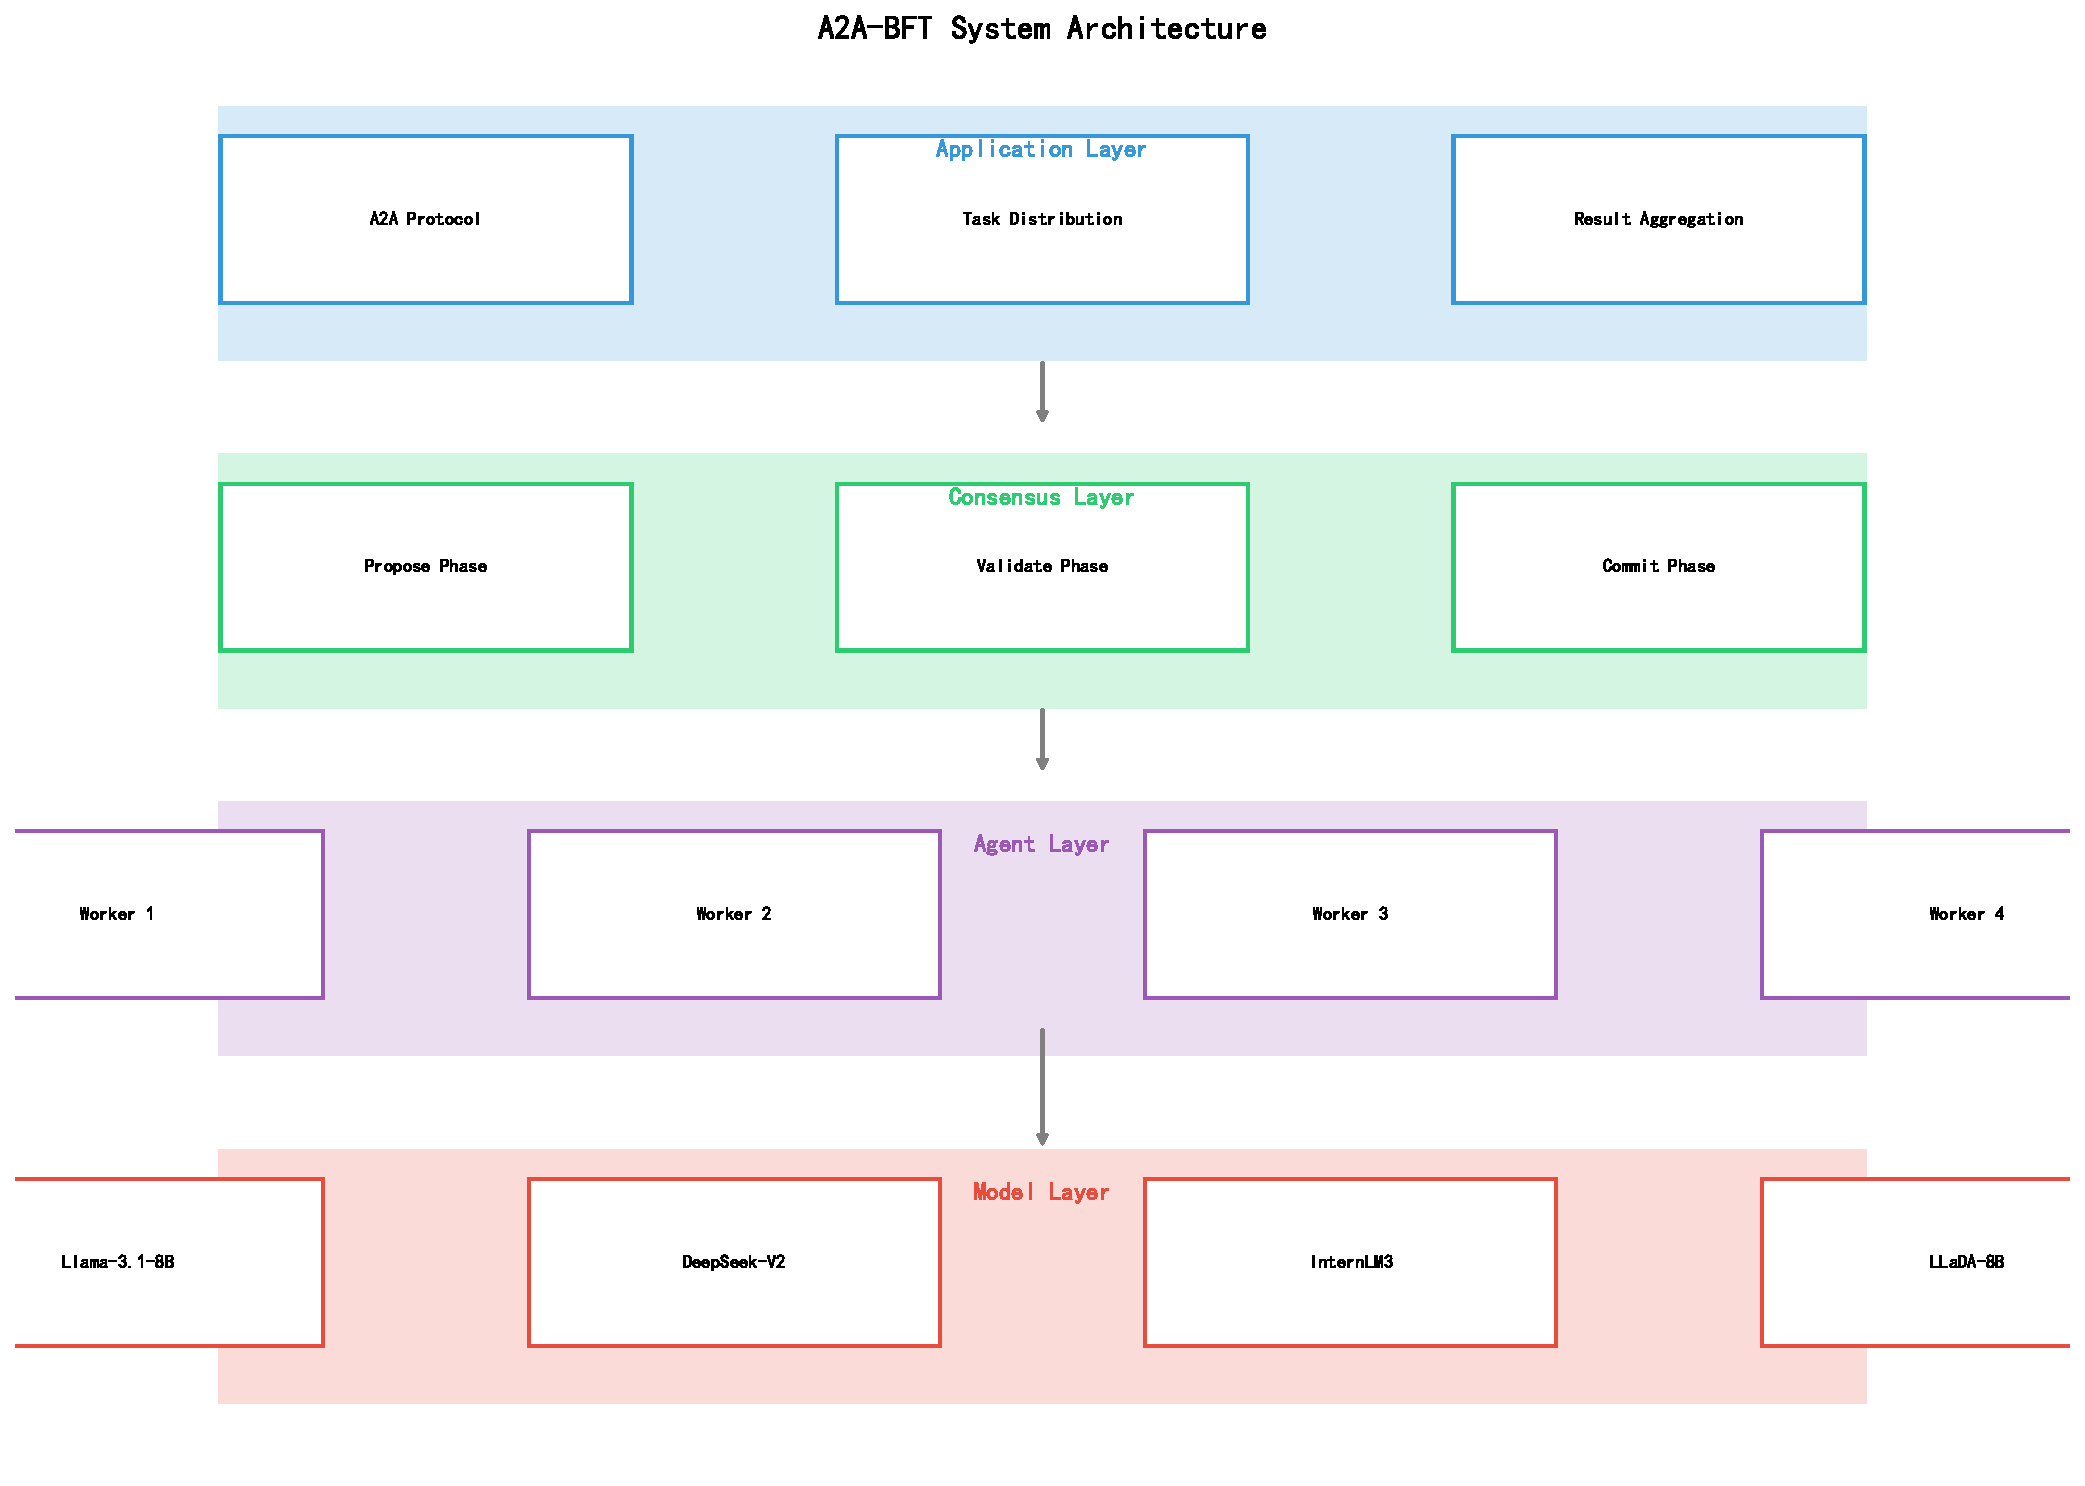
\includegraphics[width=0.9\linewidth]{figures/architecture.pdf}
\caption{A2A-BFT System Architecture}
\label{fig:architecture}
\end{figure}

\textbf{Agent Layer:} Each agent implements the DistributedWorker interface with:
\begin{itemize}
    \item Task solving capability (LLM inference)
    \item Proposal generation
    \item Independent verification
    \item Vote signing and broadcasting
\end{itemize}

\textbf{Consensus Layer:} Manages the three-phase protocol, threshold computation, and reputation tracking.

\textbf{Model Validator:} Automatically tests model quality across mathematical reasoning, logic, translation, and knowledge tasks before deployment.

\textbf{Network Layer:} Handles A2A protocol communication with message authentication and ordering.

\subsubsection{Model Integration}

A2A-BFT supports multiple LLM backends deployed on GPU infrastructure:
\begin{itemize}
    \item \textbf{Llama-3.1-8B-Instruct} \citep{meta2024llama}: General-purpose reasoning
    \item \textbf{DeepSeek-V2-Lite} \citep{deepseek2024}: Cost-effective alternative
    \item \textbf{InternLM3-8B} \citep{internlm2024}: Strong coding capability
    \item \textbf{Qwen2.5-7B-Instruct} \citep{qwen2024qwen}: General-purpose reasoning, strong code capability
\end{itemize}

Each model undergoes validation testing before deployment, ensuring minimum quality thresholds.

\subsubsection{Reputation Implementation}

The reputation tracker maintains:
\begin{itemize}
    \item Per-agent reputation scores (initialized to 1.0)
    \item Voting history (last 10 rounds) for the reject ratio $\rho_i$
    \item Suspect counters for anomaly detection. The released code \emph{does} escalate: once a counter reaches its threshold the score is \emph{set} to $\max(0.3,\, r_i - 0.2)$, i.e.\ a further clamped decrement of $0.2$ applied to the post-tier value (an assignment, not an additive term). A step-by-step fidelity audit against the released penalty code ($12{,}000$ update steps over all three vote types, zero divergence) confirms that the escalation fires. There is no exclusion or reweighting.
    \item A correctness predicate $c$ for vote scoring. Algorithm~\ref{alg:reputation} requires ``is the proposal correct''; the released \texttt{\_estimate\_correctness} approximates this with a format check (a final-answer marker on GSM8K, a Python code block on MBPP), evaluated on the \emph{full} model response rather than a prefix---truncating the response would flip the predicate on answers whose marker appears late. Section~\ref{sec:rep_ablation} measures that this predicate is a per-domain constant in practice across all $457$ logged proposal rounds.
\end{itemize}

\subsection{Real LLM Validation Details}\label{app:realllm}

We conducted comprehensive experiments using the DeepSeek-V2-Lite API to validate A2A-BFT with real LLM outputs. This evaluation uses a \emph{homogeneous} single-model deployment, which upper-bounds validation agreement relative to the heterogeneous sweep; it covers 320 tasks across three domains: mathematical reasoning (GSM8K), knowledge QA (MMLU), and code generation (MBPP).

\begin{table}[htbp]
\centering
\caption{Real LLM Experiment Results (DeepSeek-V2-Lite; GSM8K, MMLU, MBPP; 320 tasks, of which 291 completed---acceptance computed over completed tasks; see the note below)}
\label{tab:real_llm}
\begin{tabular}{lcccc}
\toprule
\textbf{Configuration} & \textbf{Tasks} & \textbf{Accept\%} & \textbf{Avg Time (s)} \\
\midrule
Math baseline ($n=4,f=0,s=0$) & 40 & \textbf{100} & 6.30 \\
Math BFT ($n=5,f=1,s=1$) & 40 & \textbf{100} & 9.22 \\
Math + Strategic Reject ($n=5,f=1,s=1$) & 40 & \textbf{100} & 8.90 \\
Math + Collusion ($n=6,f=2,s=0$) & 40 & \textbf{100} & 8.49 \\
Knowledge baseline ($n=4,f=0,s=0$) & 40 & \textbf{100} & 27.00 \\
Knowledge BFT ($n=5,f=1,s=1$) & 40 & \textbf{100} & 28.13 \\
Code baseline ($n=4,f=0,s=0$) & 40\,(12)$^\star$ & \textbf{100} & 38.16 \\
Code BFT ($n=5,f=1,s=1$) & 40\,(39)$^\star$ & \textbf{100} & 9.01 \\
\midrule
\textbf{Total} & \textbf{320} & \textbf{100} & -- \\
\bottomrule
\end{tabular}
\end{table}

\textbf{Key Findings:}
\begin{enumerate}
    \item A2A-BFT achieves high acceptance rate across all task types with real LLM outputs, confirming cross-domain portability of the consensus protocol.
    \item Byzantine attacks (strategic rejection, collusion) are resisted without impacting honest agent consensus.
    \item Inference latency is dominated by LLM generation and varies by task type: math ($\sim$6.3--9.2s), knowledge ($\sim$27--28s), code ($\sim$9--38s).
    \item No proposal was rejected by the protocol in any configuration; every non-acceptance is an API/harness failure (see the note below).
\end{enumerate}

\textbf{Note on Table~\ref{tab:real_llm}:} $^\star$The ``Tasks'' column shows submitted (and, in parentheses, completed) tasks: $28$ code-baseline tasks and $1$ code-BFT task terminated in API/harness errors, and $100\%$ is computed over the completed ones. All 320 tasks were submitted to the live DeepSeek API, and acceptance is computed over the $291$ that completed execution---every one was accepted. The other $29$ terminated in API/harness errors ($28$ in the code-baseline row, whose wall-clock is inflated to $38.16$s; $1$ in the code-BFT row) and are excluded. No proposal was \emph{rejected} in any configuration ($\texttt{reject\_count}=0$), so the $100\%$ column reflects consensus, not filtering, and every latency is a genuine end-to-end measurement---the sole caveat being the code-baseline average noted above, which those $28$ terminations inflate. This table is a homogeneous-deployment upper bound (Section~6.4); the authoritative adversarial-boundary results---real Byzantine tampering, numerical verification, measured rounds---are in Table~\ref{tab:n8_scaling}.

\textbf{Measuring Answer Correctness.} A consensus protocol can reach agreement on an answer that is nonetheless wrong. To validate the \emph{validity} (not merely the \emph{agreement}) guarantee of A2A-BFT, we additionally measure answer correctness: for each accepted proposal we extract the final numerical answer and compare it against the GSM8K ground truth. This distinguishes a protocol that merely terminates from one that terminates on the \emph{correct} answer. The results (Table~\ref{tab:n8_scaling}) show that under Byzantine attacks the consensus rate remains at or near $100\%$ ($98$--$100\%$ across two independent runs), while answer correctness stays within a statistically insignificant margin of the fault-free baseline ($92.0$--$92.7\%$ vs.\ $94.0\%$). The decisive evidence of genuine resistance is the round-count gap ($1.03$ vs.\ $2.89$--$2.92$ rounds; Welch $t \leq -13.1$, $p < 10^{-26}$): Byzantine primaries tamper with answers, honest validators reject them, and view change rotates to an honest primary before a correct answer is accepted. This gap is reproduced in a repeat run ($1.04$ vs.\ $2.38$--$2.43$ rounds), whereas the consensus rate there is $100\%$; the paired per-task difference between the two runs is not significant (McNemar exact $p = 0.25$ on each attacked configuration, computed over the identical task sets), so we report the more conservative run and treat the residual decision-rate variation as API run-to-run variance.

The full performance trade-off analysis and statistical significance tests, the complete attack-resistance breakdown, and the direct comparison with A2A-Sim under identical conditions are provided in Appendix~\ref{app:additional}.

\subsection{Additional Experimental Analysis}\label{app:additional}

Tables~\ref{tab:baseline}, \ref{tab:ablation}, and \ref{tab:hetero_compare} report the fault-free baseline grid and the full ablation and baseline-comparison grids referenced in Section~\ref{sec:experiments}.

\begin{table}[htbp]
\centering\small
\caption{Baseline Performance Without Faults (real heterogeneous 4-model deployment; cells: decision\% / wrong-commit\%, mean$\pm$std over sampling seeds). $n{=}250$ tasks per cell (5 seeds $\times$ 50 tasks) except $n{=}5$ rows ($n{=}90$; 3 seeds $\times$ 30 tasks, from the ablation study deployment).}
\label{tab:baseline}
\begin{tabular}{lcccc}
\toprule
\textbf{Configuration} & \multicolumn{2}{c}{\textbf{GSM8K (semantic)}} & \multicolumn{2}{c}{\textbf{MBPP (execution)}} \\
\cmidrule(lr){2-3} \cmidrule(lr){4-5}
 & decision\% & wrong-commit\% & decision\% & wrong-commit\% \\
\midrule
$n=4, f=0, s=0$ & $59.2 \pm 9.4$ & $1.2 \pm 1.1$ & $73.2 \pm 6.1$ & $\mathbf{0.0 \pm 0.0}$ \\
$n=5, f=0, s=0$ & $56.7 \pm 5.8$ & $1.1 \pm 1.9$ & $70.0 \pm 11.5$ & $\mathbf{0.0 \pm 0.0}$ \\
$n=6, f=0, s=0$ & $55.2 \pm 7.6$ & $1.2 \pm 1.1$ & $73.6 \pm 6.5$ & $\mathbf{0.0 \pm 0.0}$ \\
\bottomrule
\end{tabular}
\end{table}

\begin{table}[htbp]
\centering
\caption{Ablation Study under Byzantine Attacks (Heterogeneous 4-Model vLLM; mean$\pm$std over three sampling seeds, 30 tasks each, $n{=}90$ per cell; cells: decision\% / wrong-commit\%). Bold marks the \emph{worst} value per column among ablation variants.}
\label{tab:ablation}
\setlength{\tabcolsep}{2pt}
\footnotesize
\begin{tabular}{lcccc}
\toprule
\textbf{Variant} & \multicolumn{2}{c}{\textbf{GSM8K (semantic)}} & \multicolumn{2}{c}{\textbf{MBPP (execution)}} \\
\cmidrule(lr){2-3} \cmidrule(lr){4-5}
 & $n{=}5,f{=}1,s{=}1$ & $n{=}8,f{=}2,s{=}1$ & $n{=}5,f{=}1,s{=}1$ & $n{=}8,f{=}2,s{=}1$ \\
\midrule
Full protocol & $74.4{\pm}8.4$/$4.5{\pm}3.9$ & $61.1{\pm}10.7$/$10.0{\pm}3.3$ & $70.0{\pm}11.5$/$\mathbf{0.0{\pm}0.0}$ & $60.0{\pm}8.8$/$\mathbf{0.0{\pm}0.0}$ \\
No View Change & $\mathbf{4.5{\pm}3.9}$/$4.5{\pm}3.9$ & $\mathbf{12.2{\pm}5.1}$/$12.2{\pm}5.1$ & $\mathbf{0.0{\pm}0.0}$/$0.0{\pm}0.0$ & $\mathbf{0.0{\pm}0.0}$/$0.0{\pm}0.0$ \\
No Sem.\ Validation & $54.4{\pm}8.4$/$2.2{\pm}1.9$ & $44.5{\pm}10.7$/$2.2{\pm}1.9$ & $\mathbf{1.1{\pm}1.9}$/$0.0{\pm}0.0$ & $\mathbf{0.0{\pm}0.0}$/$0.0{\pm}0.0$ \\
Fixed Threshold & $\mathbf{0.0{\pm}0.0}$/$0.0{\pm}0.0$ & $38.9{\pm}7.7$/$0.0{\pm}0.0$ & $\mathbf{0.0{\pm}0.0}$/$0.0{\pm}0.0$ & $51.1{\pm}13.4$/$0.0{\pm}0.0$ \\
\bottomrule
\end{tabular}
\end{table}

\begin{table}[htbp]
\centering
\caption{Baseline Comparison under Byzantine Attacks (Heterogeneous 4-Model vLLM; mean over three sampling seeds, $n{=}90$ per cell). Cells report decision\% / answer-correctness\% / wrong-commit\%; bold marks the \emph{worst} wrong-commit rate per column; seed-level std is at most 16.8 points (0--13.5 for wrong-commit), full mean$\pm$std in released data. LLM-Debate uses two debate rounds with a majority commit and no execution oracle; an oracle-assisted variant is reported in Appendix~\ref{app:attacks}.}
\label{tab:hetero_compare}
\begin{tabular}{lcccc}
\toprule
\textbf{Method} & \multicolumn{2}{c}{\textbf{GSM8K}} & \multicolumn{2}{c}{\textbf{MBPP}} \\
\cmidrule(lr){2-3} \cmidrule(lr){4-5}
 & Strat.\ Reject & Collusion & Strat.\ Reject & Collusion \\
\midrule
\textbf{A2A-BFT (ours)} & $74.4/70.0/\mathbf{4.5}$ & $61.1/51.1/\mathbf{10.0}$ & $70.0/70.0/\mathbf{0.0}$ & $60.0/60.0/\mathbf{0.0}$ \\
Simple Majority & $100/71.1/\mathbf{28.9}$ & $100/66.7/33.3$ & $100/43.3/56.7$ & $100/38.9/\mathbf{61.1}$ \\
Weighted Majority & $100/71.1/28.9$ & $100/68.9/31.1$ & $100/51.1/48.9$ & $100/45.6/54.4$ \\
A2A-Sim & $62.2/54.4/7.8$ & $66.7/58.9/7.8$ & $82.2/46.7/35.5$ & $83.3/48.9/34.4$ \\
LLM-Debate & $100/82.2/17.8$ & $100/83.3/16.7$ & $100/43.3/\mathbf{56.7}$ & $100/36.6/\mathbf{63.4}$ \\
\bottomrule
\end{tabular}
\end{table}


\subsubsection{Adversarial-Boundary Scaling ($n{=}8$, Real DeepSeek API)}
These homogeneous-API runs are an upper bound on decision rates (Section~6.4); Table~\ref{tab:n8_scaling} details answer correctness at the boundary configuration.

\begin{table}[htbp]
\centering
\caption{Answer Correctness at the Adversarial Boundary $n{=}8$ (Real DeepSeek API, GSM8K, 150 tasks per configuration). Raw per-task logs: \texttt{experiments/results/correctness\_50x3\_log.txt}. A repeat run gave $100.0/93.3/2.43$, $100.0/94.0/2.38$, $100.0/94.0/1.04$ for the three rows; the round-count gap is reproduced, the decision-rate delta is within API run-to-run variance.}
\label{tab:n8_scaling}
\begin{tabular}{lccc}
\toprule
\textbf{Configuration} & \textbf{Consensus\%} & \textbf{Correctness\%} & \textbf{Rounds} \\
\midrule
$n{=}8, f{=}2, s{=}1$ + Collusion & $98.0$ & $92.7$ & $2.89$ \\
$n{=}8, f{=}2, s{=}1$ + Strategic Reject & $98.0$ & $92.0$ & $2.92$ \\
$n{=}8, f{=}0, s{=}0$ (baseline) & $100.0$ & $94.0$ & $1.03$ \\
\bottomrule
\end{tabular}
\end{table}

\subsubsection{MMLU (Knowledge QA) Fault Sweep}
Table~\ref{tab:mmlu_sweep} completes the fault sweep of Table~\ref{tab:bft} with the knowledge-QA domain (MMLU, three core subjects; $n{=}250$ per cell).

\begin{table}[htbp]
\centering
\caption{MMLU Fault Sweep (real heterogeneous 4-model deployment; cells: decision\% / wrong-commit\%, mean$\pm$std over 5 seeds, 50 tasks each). $^\dag$: below the safety boundary.}
\label{tab:mmlu_sweep}
\begin{tabular}{ccclcc}
\toprule
\textbf{n} & \textbf{f} & \textbf{s} & \textbf{Attack} & \textbf{decision\%} & \textbf{wrong-commit\%} \\
\midrule
4 & 0 & 0 & baseline & $14.8 \pm 5.6$ & $3.6 \pm 2.6$ \\
5 & 0 & 0 & baseline & $14.8 \pm 5.9$ & $4.4 \pm 2.6$ \\
6 & 0 & 0 & baseline & $11.2 \pm 5.6$ & $2.8 \pm 1.8$ \\
4 & 1 & 0 & Random & $65.2 \pm 2.7$ & $35.6 \pm 3.6$ \\
4 & 1 & 0 & Strat.\ Reject & $73.2 \pm 7.2$ & $60.8 \pm 8.6$ \\
4 & 1 & 0 & Sybil & $68.4 \pm 6.2$ & $39.6 \pm 6.2$ \\
5 & 1 & 1 & Random & $75.2 \pm 1.8$ & $40.8 \pm 5.0$ \\
5 & 2 & 0 & Random$^\dag$ & $88.8 \pm 4.8$ & $55.6 \pm 6.1$ \\
5 & 2 & 0 & Strat.\ Reject$^\dag$ & $94.8 \pm 2.7$ & $85.2 \pm 7.9$ \\
5 & 2 & 0 & Collusion$^\dag$ & $96.0 \pm 2.0$ & $90.0 \pm 3.7$ \\
6 & 2 & 0 & Collusion$^\dag$ & $85.2 \pm 4.6$ & $74.4 \pm 7.0$ \\
\bottomrule
\end{tabular}
\end{table}

MMLU is the most demanding domain and the results are correspondingly stark. \emph{Fault-free}, only $11$--$15\%$ of tasks are decided: the subjects are hard enough that heterogeneous 8B replicas rarely agree, and the protocol correctly withholds commitment rather than gamble on an unvalidated majority. \emph{Under attack}, decision rates rise to $65$--$96\%$ (Byzantine primaries inject a stream of proposals; eventual acceptance commits whichever clears validation) and wrong commits reach $56$--$90\%$ below the boundary. This is the clearest demonstration of the oracle-composition principle: consensus safety cannot exceed validation reliability, and on hard knowledge questions 8B semantic judges are unreliable validators. The practical implication is architectural rather than negative: for knowledge-QA deployment, the Validate stage should be backed by retrieval or stronger verifier models, and the protocol's contribution is to make this requirement \emph{measurable} (wrong-commit rate) rather than invisible.

\subsubsection{Performance Analysis}
Table \ref{tab:performance} reports the real end-to-end cost of the protocol on the four-model deployment (measured wall-clock per task, including all LLM inference, validation, and view changes).

\begin{table}[htbp]
\centering
\caption{Real End-to-End Cost per Task (heterogeneous 4-model vLLM, $n{=}250$ tasks per cell). ``Calls'' counts LLM requests per task; MBPP validation executes code locally instead of invoking the judge, hence its far lower call count. GSM8K CoT generation dominates the latency.}
\label{tab:performance}
\begin{tabular}{lcccc}
\toprule
\textbf{Configuration} & \textbf{Domain} & \textbf{Time/Task} & \textbf{Calls/Task} & \textbf{Rounds} \\
\midrule
$n=4, f=0, s=0$ & GSM8K & $61.3$s & $12.7$ & $3.20$ \\
 & MBPP & $11.9$s & $2.6$ & $2.60$ \\
$n=4, f=1, s=0$ Strat.\ Reject & GSM8K & $88.0$s & $13.4$ & $3.90$ \\
 & MBPP & $14.8$s & $3.4$ & $3.40$ \\
$n=5, f=2, s=0$ Collusion$^\dag$ & GSM8K & $72.1$s & $11.0$ & $2.90$ \\
 & MBPP & $19.3$s & $4.5$ & $4.50$ \\
$n=6, f=0, s=0$ & GSM8K & $88.4$s & $20.0$ & $3.30$ \\
 & MBPP & $15.4$s & $2.6$ & $2.60$ \\
\bottomrule
\end{tabular}
\end{table}

\textbf{Cost structure:} latency is dominated by LLM generation, and it tracks the number of generations: the $n{=}4 \to n{=}6$ increase ($61.3 \to 88.4$s on GSM8K) accompanies $12.7 \to 20.0$ LLM calls per task, a linear growth in the validator count rather than the $O(n^2)$ message complexity. Attacks raise latency only moderately within the boundary ($61.3 \to 88.0$s under strategic rejection); the sub-boundary collusion row is \emph{faster} ($2.90$ vs.\ $3.20$ rounds) because colluding validators accept immediately---precisely why it is unsafe.

Figure \ref{fig:performance_comparison} shows the performance trade-offs across configurations.

\begin{figure}[htbp]
\centering
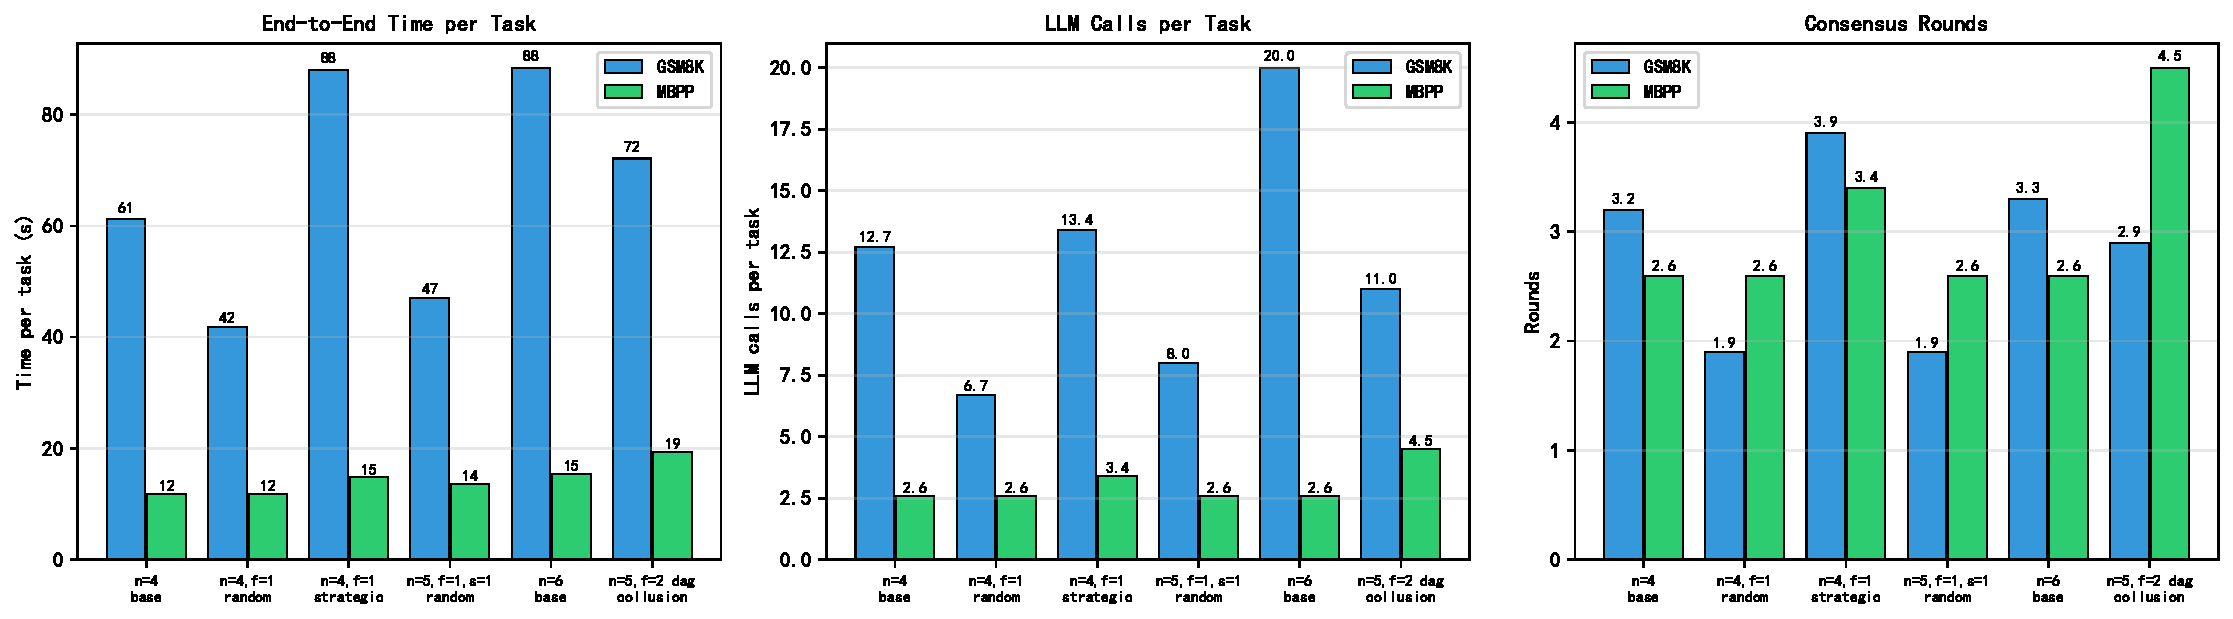
\includegraphics[width=0.85\linewidth]{figures/performance_comparison.pdf}
\caption{Real End-to-End Cost per Task (heterogeneous 4-model deployment): wall-clock time, LLM calls, and consensus rounds across representative configurations. GSM8K CoT generation dominates latency; MBPP execution validation requires far fewer LLM calls.}
\label{fig:performance_comparison}
\end{figure}

\subsection{Reputation Tracker: Full Measurement Details}\label{app:rep_details}

This appendix expands Section~\ref{sec:rep_ablation} with the full measured table, the per-finding numbers, and the complete repair analysis.

The reputation tracker is excluded from the vote-counting rule (Equation~\ref{eq:commit}; Section~\ref{sec:rep_ablation}), so a reputation-on/off comparison of decision metrics would return an identity by Theorem~\ref{thm:safety}; we instead measure \emph{what the tracker reports}. We instrumented the protocol to log every validation vote from the same four-model deployment (single sampling seed; 20 tasks per cell over the six scenarios of Table~\ref{tab:ablation}; 120 consensus runs, 457 scored proposal rounds, and 2{,}461 scored validation events, where one \emph{event} is one reputation update triggered by one validation vote) and replayed the recorded vote streams offline through Algorithm~\ref{alg:reputation} under four settings: $c$ taken from ground truth (\emph{oracle}; the definition Algorithm~\ref{alg:reputation} requires) or from the released \texttt{\_estimate\_correctness} heuristic (\emph{released}); and reputation persisting across tasks, as in the reference implementation where one consensus layer lives for the whole run, or reset per task. Replay issues no LLM calls and is therefore exactly reproducible; in \emph{all four} settings the replayed decision sequence is identical to the online record, which is both a correctness check and direct evidence that no reported decision depends on the tracker. Table~\ref{tab:rep_ablation} reports the oracle/persistent setting.

\begin{table}[htbp]
\centering
\caption{Measured reputation-tracker behaviour (oracle $c$, persistent reputation; single seed, 20 tasks per cell). \emph{Aggr.} = aggressive-tier events ($\rho_i \geq 0.7$, $-0.25$); one event is one reputation update triggered by one validation vote, so events are \emph{not} independent observations. \emph{Mis-pen.} = aggressive penalties landing on an honest validator whose vote was \emph{objectively correct}---the case Section~\ref{sec:reputation} specifies should be rewarded. Pre./Rec.\ treat an aggressive penalty as a Byzantine detector. \emph{Escal.\ $\to$ hon.} = fraction of suspect-counter escalations ($-0.2$) landing on honest agents. $r$ = mean end-of-task reputation, averaged over all (task, validator) snapshots in the cell; ``---'' = the cell contains no Byzantine validator.}
\label{tab:rep_ablation}
\setlength{\tabcolsep}{3.5pt}
\footnotesize
\begin{tabular}{lrrrrrrr}
\toprule
\textbf{Scenario} & \textbf{Aggr.} & \textbf{Mis-pen.} & \textbf{Rate} & \textbf{Pre.} & \textbf{Rec.} & \textbf{Escal.\ $\to$ hon.} & \textbf{$r$ hon./Byz.} \\
\midrule
GSM8K $f{=}0$ (no attack) & 66 & 42 & 0.636 & --- & --- & 1.000 & 0.587\,/\,--- \\
GSM8K $f{=}1$ strat.\ rej. & 164 & 116 & 0.707 & 0.232 & 1.000 & 0.832 & 0.436\,/\,0.300 \\
GSM8K $f{=}2$ collusion & 373 & 355 & \textbf{0.952} & \textbf{0.000} & \textbf{0.000} & 0.856 & \textbf{0.337\,/\,0.427} \\
MBPP $f{=}0$ (no attack) & 88 & 88 & 1.000 & --- & --- & 1.000 & 0.573\,/\,--- \\
MBPP $f{=}1$ strat.\ rej. & 200 & 155 & 0.775 & 0.195 & 1.000 & 0.843 & 0.338\,/\,0.332 \\
MBPP $f{=}2$ collusion & 568 & 560 & \textbf{0.986} & \textbf{0.000} & \textbf{0.000} & 0.888 & \textbf{0.300\,/\,0.412} \\
\bottomrule
\end{tabular}
\end{table}

Four findings, from descriptive single-seed measurements ($20$ tasks per cell; see Limitations). \textbf{(i) The aggressive tier fires almost exclusively on honest, correct votes.} Across the four cells containing Byzantine validators, $1{,}186$ of $1{,}305$ aggressive penalties landed on an honest validator whose vote was objectively correct---exactly the behaviour Section~\ref{sec:reputation} specifies should be \emph{rewarded}. Reputation updates are clustered within validators and tasks, so we do not attach a binomial interval to that ratio; the task-level statistic is unambiguous: \emph{all 20 tasks} in each of the four attacked cells produced at least one mis-penalty. The mechanism is structural: honest validators correctly reject the wrong proposals that Byzantine primaries inject, so their own rejection ratio $\rho_i$ climbs past $0.7$ and the $\rho$-keyed tier overrides the reward branch. In the two cells with \emph{no} Byzantine validator at all the tier still fires (66 and 88 events, in 10 and 9 of 20 tasks respectively, of which 8 and 9 produced a mis-penalty---a penalty on an honest, correct vote in a cell where no adversary exists), because disagreeing with a wrong proposal is itself what raises $\rho_i$. \textbf{(ii) As a Byzantine detector the tier fails.} Treating an aggressive penalty as a Byzantine flag yields recall $1.000$ but precision $0.232$/$0.195$ under strategic rejection, and \emph{precision and recall both $0.000$} under collusion. The logged $\rho_i$ makes the mechanism explicit: a colluding validator rejects only in the round where an honest primary's proposal is finally committed, so its mean rejection ratio stays at $0.358$ (GSM8K) and $0.392$ (MBPP) and never reaches the $0.7$ trigger in a single validator-task pair, whereas honest validators---who must reject the wrong proposals those same primaries inject---average $0.600$ and $0.851$, crossing $0.7$ in $61.7\%$ and $90.0\%$ of pairs. Under strategic rejection, by contrast, Byzantine validators reject unconditionally ($\bar\rho = 1.000$, $1.9$ aggressive hits per task) and are caught, which is why recall is $1.000$ there. \textbf{(iii) The score ordering inverts.} In both collusion cells honest validators finish \emph{below} Byzantine ones ($0.337$ vs.\ $0.427$ on GSM8K; $0.300$ vs.\ $0.412$ on MBPP; Figure~\ref{fig:reputation}, right), the opposite of the accountability ordering the tracker is meant to produce. Resetting reputation per task does not repair this (honest $0.391$ vs.\ Byzantine $0.761$ on GSM8K collusion), so the failure is structural rather than a cold-start artefact. \textbf{(iv) The released $c$ carries negative information.} Algorithm~\ref{alg:reputation} requires $c$ = ``is the proposal correct''. The released \texttt{\_estimate\_correctness} is a format check that returns \texttt{False} for all $241$ GSM8K rounds and \texttt{True} for all $216$ MBPP rounds---a per-domain constant. It is not merely uninformative but counter-productive: the base rate of correct proposals across all $457$ rounds is $25.4\%$, so the trivial always-\texttt{False} predictor would agree with ground truth $74.6\%$ of the time, whereas the released predicate---constant within each domain---agrees on only $46.2\%$. On GSM8K it happens to pick the better of the two constants ($69.7\%$ vs.\ $30.3\%$ for always-\texttt{True}); on MBPP it picks the worse one ($19.9\%$ vs.\ $80.1\%$). Overall it is worse than the cheapest possible baseline. In the released configuration the reward and mild-penalty tiers are therefore driven by vote \emph{direction} alone, and the promised reward for correctly rejecting a wrong proposal does not occur.

Two conclusions follow. First, the tracker is genuinely decision-neutral: recomputing $\phi$ from the raw votes reproduces all $457$ recorded rounds and replaying the vote-and-threshold state machine reproduces all $120$ online decisions together with the primary rotation, whereas a mutation that injects reputation weights shifts $\phi$ in up to $421$ rounds and flips up to $5$ decisions---a check that can fail rather than a tautology. Second, as an incentive mechanism the released tracker is mis-specified: it taxes precisely the behaviour it is meant to encourage. Because no reported safety or liveness \emph{number} depends on it, the quantitative results stand; but the deterrent that Appendix~\ref{app:attack_resistance} lists against strategic rejection is not delivered by the released code, so that entry should be read as specified rather than realised. This failure mode is itself known to the trust literature---reputation rules keyed on a rater's own behaviour punish honest negative feedback \citep{josang2002beta,josang2007survey}, and P2P designs such as EigenTrust \citep{kamvar2003eigentrust} inherit the same exposure. What we add is the scale of the effect in a real LLM consensus deployment ($1{,}186/1{,}305$ mis-attributed penalties; $20/20$ affected tasks in every attacked cell) and evidence that it is structural rather than a tuning artefact.

Repairing it requires (a) a correctness oracle for $c$ that measures the \emph{proposal} rather than its surface form, and (b) a trigger that is a function of the proposal's validated quality rather than of the validator's own rejection ratio, which honest disagreement inflates. We deliberately do \emph{not} suggest keying the trigger on agreement with the committee's majority: that would reintroduce exactly the coupling to the committee's decision that Algorithm~\ref{alg:reputation} is designed to avoid, and under attack it would penalise precisely the lone correct dissenters the mechanism exists to protect. Triggers compatible with this constraint include execution-validated outcomes on verifiable domains and DID-signed cross-round consistency on semantic ones. We leave the repaired design to future work; the instrumented vote streams and the four-setting replay are released for independent verification.

Figure \ref{fig:reputation} depicts the reputation update rule (Algorithm~\ref{alg:reputation}) alongside \emph{measured} per-agent reputation trajectories from the real four-model deployment (Section~\ref{sec:rep_ablation}); the trajectories are replay-derived from the instrumented vote streams (Algorithm~\ref{alg:reputation} re-executed offline on the logged votes), so the right panel is measured rather than schematic.

\begin{figure}[htbp]
\centering
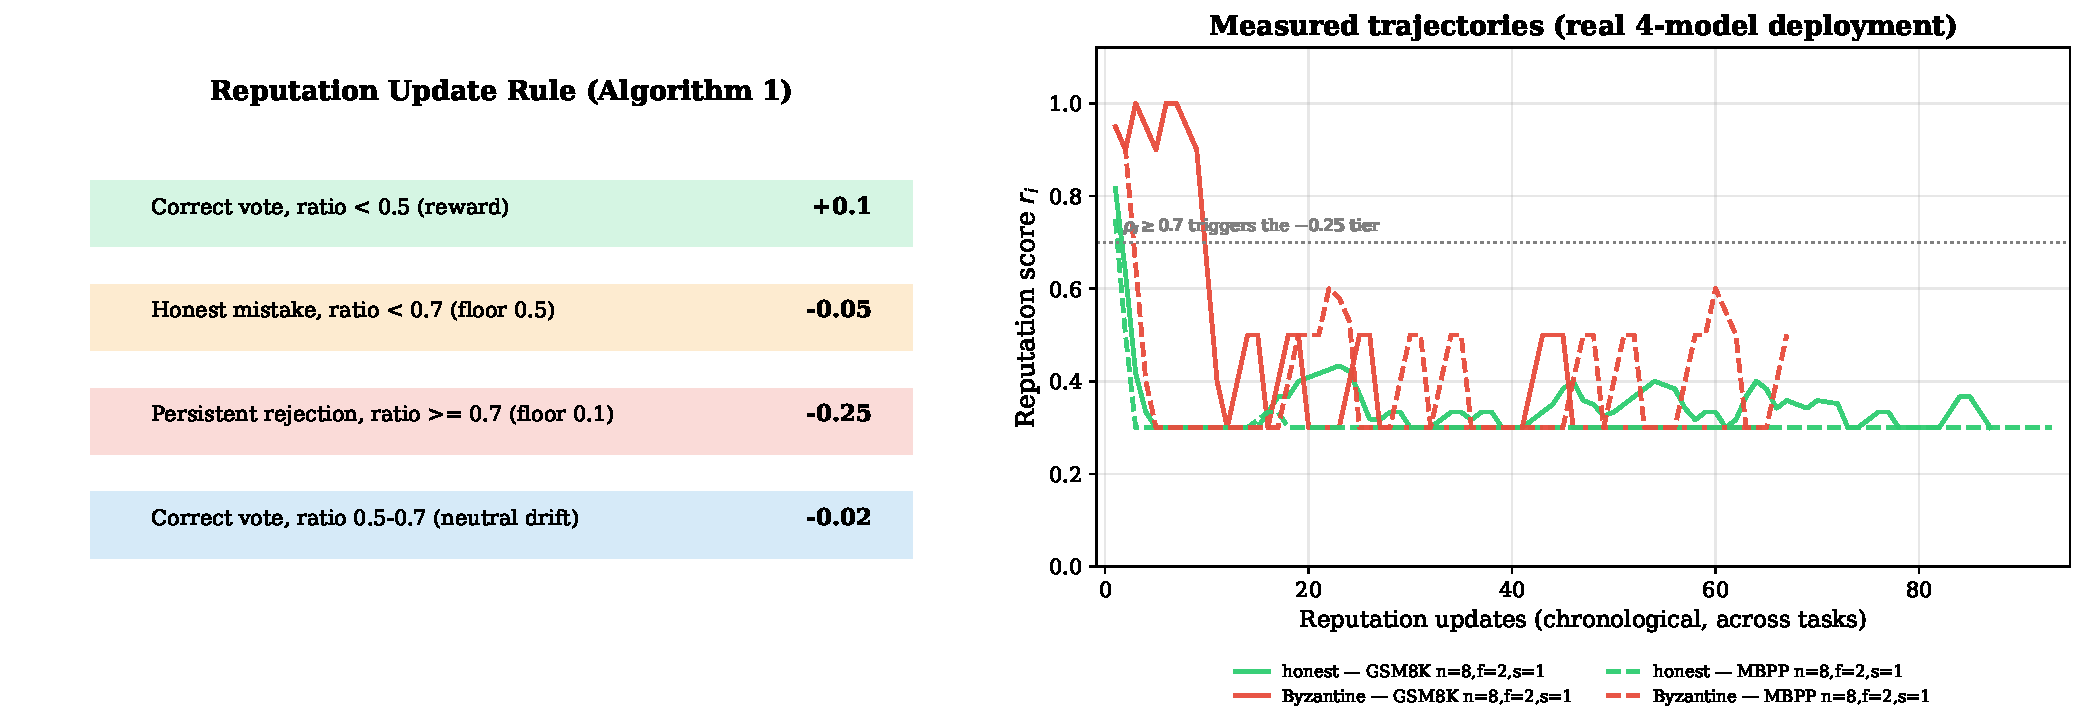
\includegraphics[width=0.75\linewidth]{figures/reputation_mechanism.pdf}
\caption{Reputation update rule (Algorithm~\ref{alg:reputation}; left) and \emph{measured} per-agent reputation trajectories under collusion in the real four-model deployment (right; replay-derived by re-executing Algorithm~\ref{alg:reputation} offline on the logged vote streams; 20 tasks per cell, oracle $c$, reputation persisting across tasks; Section~\ref{sec:rep_ablation}). In both collusion cells the honest curves finish \emph{below} the Byzantine ones.}
\label{fig:reputation}
\end{figure}


\subsection{Attack Resistance Analysis}\label{app:attack_resistance}

A2A-BFT's behavior under all tested attack vectors separates cleanly along the safety boundary:

\begin{table}[htbp]
\centering
\caption{Attack Resistance Summary (real 4-model deployment; ranges over configurations of Table~\ref{tab:bft}, $n{=}250$ per cell, plus the within-boundary collusion configuration $n{=}8,f{=}2,s{=}1$ from Table~\ref{tab:hetero_compare}, $n{=}90$ per cell). ``Boundary'' = configurations satisfying $n \geq 3f{+}s{+}1$; ``below'' = $n{=}5,f{=}2$ and $n{=}6,f{=}2$ for $f{=}2$.}
\label{tab:attacks}
\begin{tabular}{llcccc}
\toprule
 & & \multicolumn{2}{c}{\textbf{Within boundary}} & \multicolumn{2}{c}{\textbf{Below boundary}$^\dag$} \\
\cmidrule(lr){3-4} \cmidrule(lr){5-6}
\textbf{Attack} & \textbf{Type} & \textbf{decision\%} & \textbf{wrong\%} & \textbf{decision\%} & \textbf{wrong\%} \\
\midrule
Strategic Reject & Malicious & $70.0$--$80.8$ & $0.0$--$23.2$ & $74.4$--$95.2$ & $9.6$--$67.6$ \\
Collusion & Malicious & $60.0$--$61.1$ & $0.0$--$10.0$ & $66.4$--$98.4$ & $0.0$--$72.4$ \\
Sybil Attack & Malicious & $73.6$--$90.4$ & $0.0$--$12.8$ & -- & -- \\
Random Fault & Soft & $73.2$--$90.8$ & $0.0$--$14.0$ & $78.8$--$96.8$ & $5.6$--$22.0$ \\
\bottomrule
\end{tabular}
\end{table}

\textbf{Note:} Wrong-commit ranges span the two validation semantics: the lower end is always MBPP (execution validation, mechanically $0\%$ within the boundary) and the upper end is GSM8K (8B semantic judges). Within the boundary the protocol never commits a wrong answer on execution-validated tasks; on semantic tasks the wrong-commit rate is bounded by the judge's susceptibility to plausible-but-wrong proposals. Below the boundary ($f{=}2$, $n{=}5,6$, where $3f{+}s{+}1 = 7 > n$) safety is violated on both domains (up to $9.6\%$ on execution-validated code and $72.4\%$ on GSM8K)---empirically confirming that $3f{+}s{+}1$ is a tight operating condition in the evaluated regime $s \le f$, not an artifact of the analysis.

\begin{itemize}
    \item \textbf{Strategic Rejection:} Specified to be penalised by the reputation tracker (Algorithm~\ref{alg:reputation}; Figure~\ref{fig:reputation}); the four-model sweep executes with uniform weights. Section~\ref{sec:rep_ablation} measures the released tracker as a Byzantine detector at precision $0.195$--$0.232$ under strategic rejection (recall $1.000$) but $0.000$ under collusion, with the bulk of aggressive penalties landing on honest validators whose vote was objectively correct (Section~\ref{sec:rep_ablation}), so the deterrent is best read as unrealised rather than merely unmeasured.
    \item \textbf{Collusion:} Threshold design prevents coordinated Byzantine attacks from overwhelming honest consensus.
    \item \textbf{Sybil Attack:} Weight-based voting and DID authentication limit Sybil influence.
\end{itemize}

Figure \ref{fig:attack_resistance} visualizes attack resistance across configurations.

\begin{figure}[htbp]
\centering
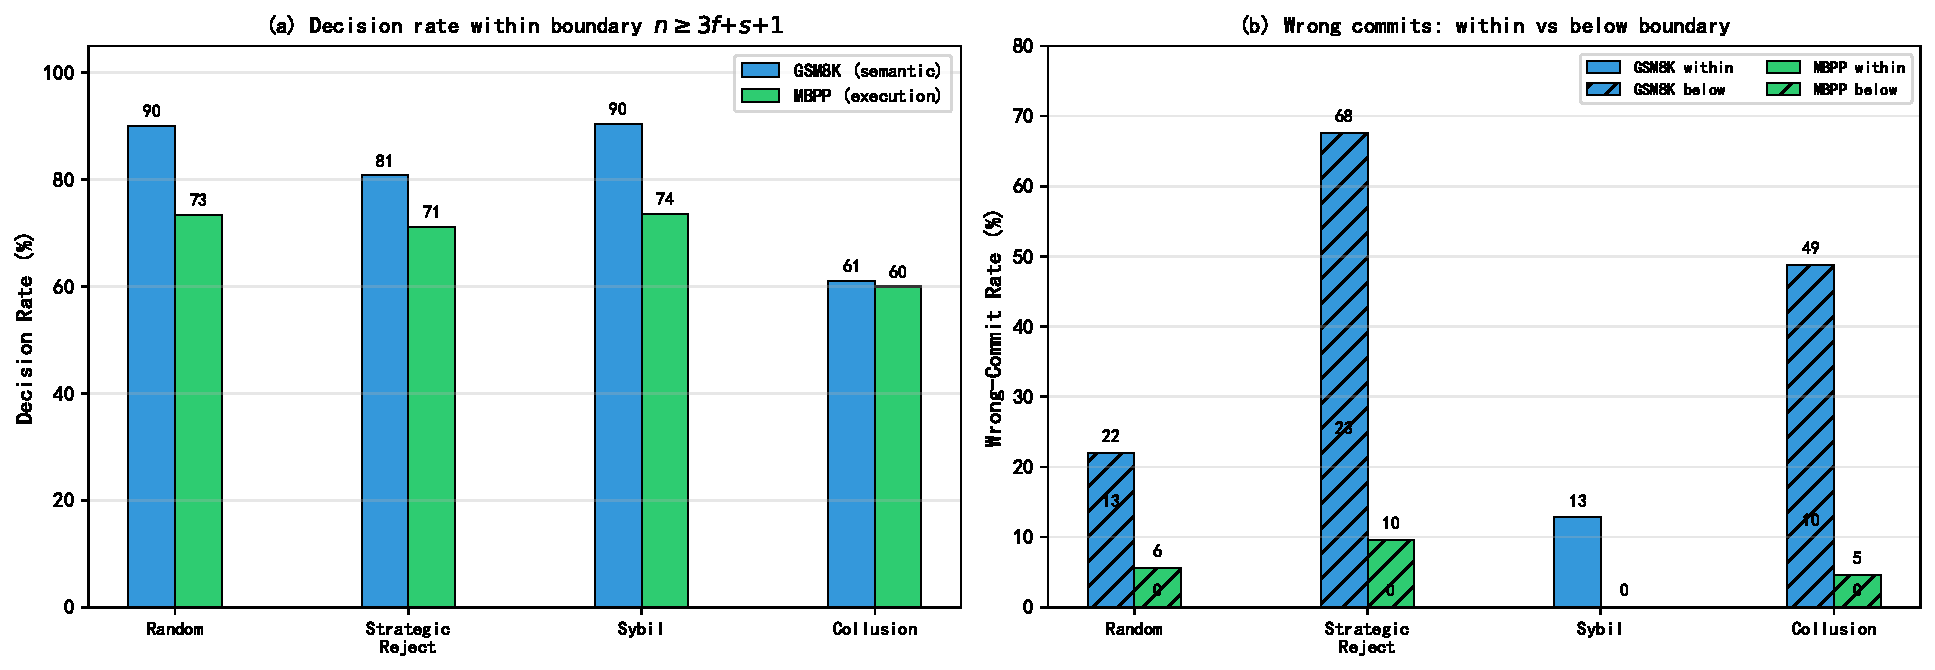
\includegraphics[width=0.78\linewidth]{figures/attack_resistance.pdf}
\caption{Attack Resistance (real 4-model deployment). Bars are from the $n{=}250$ four-model sweep, except the within-boundary collusion bars ($n{=}8,f{=}2,s{=}1$), which come from the $n{=}90$ ablation/comparison deployment (cf.\ Table~\ref{tab:attacks}). (a) Decision rates within the safety boundary. (b) Wrong-commit rates: hatched bars are sub-boundary configurations, where safety violations emerge exactly as the theorem permits.}
\label{fig:attack_resistance}
\end{figure}


\subsection{Comparison with A2A-Sim}

A2A-Sim \citep{a2a_sim_2026} provides a comprehensive evaluation of LLM agent consensus without BFT guarantees. Table \ref{tab:a2a_sim_comparison} presents a direct comparison. \textbf{Note:} Only the benign consensus rate ($41.6\%$) is quoted directly from the original publication \citep{a2a_sim_2026}; the remaining rows are computed from our heterogeneous four-model evaluation (Table~\ref{tab:hetero_compare}; 3 sampling seeds, $n{=}90$ per cell), in which an A2A-Sim-style unvalidated scalar-consensus baseline is compared under identical conditions. These rows are \emph{not} directly comparable to the original study's ``invalid consensus'' rate: the original measures agreement on a value outside the valid set in a scalar no-stake game and finds most failures to be liveness losses, whereas we measure committed answers against GSM8K/MBPP ground truth under an answer-tampering Byzantine primary.

\begin{table}[htbp]
\centering
\caption{A2A-BFT vs A2A-Sim. The benign rate is quoted from the original publication; all remaining cells (incl.\ the fault-free A2A-BFT row) use the heterogeneous four-model evaluation (3 seeds, $n{=}90$/cell; strategic rejection, GSM8K/MBPP), where $\pm$ is the seed-level std of the replication run. $^\dagger$Different metric and source---agreement rate in a scalar no-stake game, quoted from \citet{a2a_sim_2026}---so no $\Delta$ is computed for this row.}
\label{tab:a2a_sim_comparison}
\setlength{\tabcolsep}{4.5pt}
\begin{tabular}{lccc}
\toprule
\textbf{Metric} & \textbf{A2A-Sim} & \textbf{A2A-BFT} & \textbf{$\Delta$} \\
\midrule
Acceptance decision (no faults) & $41.6\%^\dagger$ & $56.7{\pm}5.8$ / $70.0{\pm}11.5\%$ & --- \\
Decision rate ($f{=}1$, strat.\ reject) & $62.2\% \pm 5.1\%$ & $74.4\% \pm 8.4\%$ & $+12.2$ pp \\
Wrong-commit ($f{=}1$ attacks) & $7.8$--$35.5\%$ & $0.0$--$4.5\%$ & $-3.3$ to $-35.5$ pp \\
\bottomrule
\end{tabular}
\end{table}

\textbf{Key Differences:}
\begin{itemize}
    \item A2A-Sim is a measurement framework rather than a protocol, so its $41.6\%$ benign rate is not a protocol deficiency but evidence that LLM agents struggle to converge on a shared value even with no faults present---the same phenomenon that caps our own fault-free GSM8K decision rate at $55$--$59\%$. What it does not provide is any guarantee once faults \emph{are} present, which is the gap A2A-BFT addresses.
    \item With one Byzantine replica under strategic rejection, A2A-Sim decides fewer tasks ($62.2\%$ vs.\ $74.4\%$) and commits wrong answers in up to $35.5\%$ of code tasks, whereas A2A-BFT never commits a wrong answer on execution-validated code ($0.0\%$).
    \item The collusion cell in Table~\ref{tab:hetero_compare} is the one place where the comparison does not favour us: at $n{=}8, f{=}2, s{=}1$ on GSM8K, A2A-Sim's decision rate is marginally higher ($66.7\%$ vs.\ $61.1\%$) and its wrong-commit rate marginally lower ($7.8\%$ vs.\ $10.0\%$). Both differences are within the $\pm$std of three seeds ($7.8{\pm}1.9$ vs.\ $4.5{\pm}3.9$ for wrong-commit under strategic rejection; descriptive at three seeds), and neither survives pooling: what separates the methods is the code domain ($34.4$--$35.5\%$ vs.\ $0.0\%$ wrong commits) and the fact that A2A-BFT's decisions carry a proof obligation rather than a confidence threshold. Under collusion the protocol is deliberately conservative---it forgoes a decision when validation is inconclusive---which costs decision rate in exactly the cell where an unvalidated aggregator happens to agree with itself.
\end{itemize}

\textbf{Design Philosophy:} While A2A-Sim focuses on evaluating LLM agent communication patterns, A2A-BFT addresses the critical gap of Byzantine fault tolerance in A2A networks. The two approaches are complementary: A2A-Sim provides insights into LLM consensus behavior, while A2A-BFT provides the theoretical guarantees necessary for production deployment.

\subsection{Rational Byzantine Analysis}\label{app:rational}

We extend the analysis to rational (rather than malicious) Byzantine agents who optimize utility rather than cause harm:

\begin{definition}[Rational Byzantine Agent]
A rational Byzantine agent maximizes expected utility $U = B - C$, where $B$ is benefit from deviation and $C$ is cost of reputation penalty.
\end{definition}

\textbf{Game-Theoretic Analysis:} Under repeated interaction with reputation tracking, honest behavior constitutes a Nash equilibrium when:
\begin{equation}
    \Delta r \cdot V_{consensus} > B_{deviation}
\end{equation}
where $\Delta r = 0.25$ is the reputation penalty for aggressive misbehavior, and $V_{consensus}$ is the value of successful consensus participation.

\begin{itemize}
    \item \textbf{Incentive Compatibility:} The reputation mechanism is \emph{designed} to create incentives for honest behavior---agents with high reputation receive more influence in future rounds. This analysis applies to the intended design, in which the penalty falls on the deviating agent; Section~\ref{sec:rep_ablation} measures the released implementation and finds the opposite (penalties land predominantly on honest, correct votes), so the equilibrium below describes a \emph{repaired} tracker rather than the one we evaluated.
    \item \textbf{Nash Equilibrium:} Under the reputation-based weight adjustment, honest behavior constitutes a Nash equilibrium when the long-term benefit of reputation exceeds the short-term gain from strategic rejection.
    \item \textbf{Repeated Game Dynamics:} The reputation tracker maintains history over the last 10 rounds, creating a repeated game context where cooperation is sustainable.
\end{itemize}

This condition is satisfied when the reputation penalty ($\Delta r = 0.25$ for aggressive misbehavior) multiplied by the consensus value exceeds any private benefit from deviation; in practice $V_{consensus}$ is large, making honest behavior the dominant strategy. The qualification is important: under the \emph{released} tracker of Section~\ref{sec:rep_ablation}, where the aggressive tier fires predominantly on honest correct votes and misses colluders entirely (precision and recall $0.000$; Section~\ref{sec:rep_ablation}), a utility-maximising agent would instead be pushed toward accepting Byzantine proposals to keep $\rho_i$ low. The repaired trigger proposed in Section~\ref{sec:rep_ablation} is a prerequisite for the equilibrium statement, not a consequence of the current code.

\subsection{Practical Deployment Considerations}\label{app:deployment}

\begin{itemize}
    \item \textbf{Network Requirements:} A2A-BFT requires authenticated channels with message ordering.
    \item \textbf{Hardware Specifications:} Two NVIDIA A800-SXM4-80GB GPUs with 512GB RAM.
    \item \textbf{Scalability:} Current implementation supports $n \leq 10$; distributed consensus optimization required for larger deployments.
\end{itemize}

\subsection{Design Trade-offs}

A2A-BFT balances several trade-offs:
\begin{itemize}
    \item \textbf{Security vs. Efficiency:} Higher fault tolerance requires more validators, increasing communication overhead.
    \item \textbf{Reactivity vs. Stability:} Fast reputation updates improve responsiveness but may cause oscillation.
    \item \textbf{Decentralization vs. Performance:} Fully decentralized operation increases latency but eliminates single points of failure.
\end{itemize}

\subsection{Future Work}

\begin{enumerate}
    \item \textbf{Adaptive Attacks:} This paper evaluates static attack patterns (strategic rejection, collusion, Sybil). Future work should explore adaptive attacks where Byzantine agents dynamically adjust behavior based on observed consensus state.
    \item \textbf{Rational Byzantine Quantification:} Appendix~\ref{app:rational} provides qualitative Nash equilibrium analysis for rational agents. Future work should add numerical simulations to validate the equilibrium conditions under different game parameters.
    \item \textbf{LLM Parameter Sensitivity:} The $p_h \geq 0.9$ assumption may not hold for all tasks or models. Future work should provide sensitivity curves showing acceptance probability across a range of $p_h$ values.
    \item \textbf{Distributed Consensus:} Current implementation is centralized; distributing the consensus layer would enable $n > 10$ deployments.
    \item \textbf{Repairing the Reputation Trigger:} Section~\ref{sec:rep_ablation} shows that the released $\rho_i$-keyed trigger mis-attributes the bulk of aggressive penalties in the attacked cells to honest validators. Future work should design and evaluate a trigger keyed on the proposal's validated quality (execution outcomes on verifiable domains, DID-signed cross-round consistency on semantic ones) and re-measure the mis-attribution rate under the same instrumented-replay protocol.
\end{enumerate}

\section{Discussion}\label{sec:discussion}

\subsection{Implications for Multi-Agent Systems}

A2A-BFT provides a foundation for reliable multi-agent collaboration under adversarial conditions. The three-phase semantic consensus design balances expressiveness with formal guarantees, while a \emph{repaired} reputation framework (Section~\ref{sec:rep_ablation}) is intended to address practical concerns about agent reliability.

\subsection{Privacy Considerations}

The protocol assumes authenticated channels, which may reveal agent identities. Potential extensions include:
\begin{itemize}
    \item Zero-knowledge proofs for private verification
    \item Differential privacy for reputation updates
    \item Secure multi-party computation for vote aggregation
\end{itemize}



\subsection{Extended Related Work}\label{app:extrelated}

\subsubsection{Byzantine Fault Tolerance in Distributed Systems}

Classical BFT protocols, beginning with PBFT \citep{castro1999practical}, establish consensus in distributed systems with Byzantine faults. Subsequent work including HotStuff \citep{yin2019hotstuff} and Tendermint \citep{buchman2018latest} improved efficiency and practicality. Foundational results establish the fundamental limits of Byzantine agreement under partial synchrony \citep{dwork1988consensus} and, in fully asynchronous settings, the $3f{+}1$ resilience bound \citep{lamport1982byzantine}. Our work extends these foundations to the LLM-based agent context.

\subsubsection{Multi-Agent Consensus with LLMs}

A2A-Sim \citep{a2a_sim_2026} provided the first systematic evaluation of LLM agent consensus, revealing only a 41.6\% success rate even in benign, no-stake settings, with failures dominated by liveness loss. Their work highlighted the gap between theoretical BFT guarantees and practical LLM behavior.

Recent approaches have explored confidence-aware and robust aggregation mechanisms. CP-WBFT \citep{zheng2025rethinking} introduces confidence probes to weight agent contributions, while SAC (Self-Anchored Consensus) \citep{lee2026robust} proposes decentralised filter-and-refine aggregation with graph-robustness conditions for Byzantine robustness of decentralised LLM agent networks. Multi-agent debate showed that structured argumentation can improve reasoning accuracy \citep{du2024improving,liang2023encouraging}, and Self-Consistency demonstrated that aggregating multiple reasoning paths reduces error rates \citep{wang2023self}. Surveys of LLM-based multi-agent systems \citep{guo2024survey} provide taxonomies of collaboration patterns; frameworks such as AutoGen \citep{wu2023autogen} study multi-agent conversation among LLM instances. However, these approaches do not address the specific challenges of A2A protocols or provide formal safety and liveness guarantees with attack-resistance experiments. Our work differs by providing formal safety and liveness guarantees for consensus in the presence of Byzantine and soft faults within the A2A protocol framework, together with an execution-validated safety metric (wrong-commit rate).

\end{document}
